%!TEX TS-program = xelatex
\documentclass[10pt,oneside]{article}
\usepackage[fontsize=9pt]{scrextend}

\usepackage[english]{babel}

\usepackage{amsmath,amssymb,amsfonts}
\usepackage[utf8]{inputenc}
\usepackage[T1]{fontenc}
\usepackage{stix2}
\usepackage[scaled]{helvet}
\usepackage[scaled]{inconsolata}

\usepackage{lastpage}

\usepackage{setspace}

\usepackage{ccicons}

\usepackage[hang,flushmargin]{footmisc}

\usepackage{geometry}

\setlength{\parindent}{0pt}
\setlength{\parskip}{6pt plus 2pt minus 1pt}

\usepackage{fancyhdr}
\renewcommand{\headrulewidth}{0pt}\providecommand{\tightlist}{%
  \setlength{\itemsep}{0pt}\setlength{\parskip}{0pt}}

\makeatletter
\newcounter{tableno}
\newenvironment{tablenos:no-prefix-table-caption}{
  \caption@ifcompatibility{}{
    \let\oldthetable\thetable
    \let\oldtheHtable\theHtable
    \renewcommand{\thetable}{tableno:\thetableno}
    \renewcommand{\theHtable}{tableno:\thetableno}
    \stepcounter{tableno}
    \captionsetup{labelformat=empty}
  }
}{
  \caption@ifcompatibility{}{
    \captionsetup{labelformat=default}
    \let\thetable\oldthetable
    \let\theHtable\oldtheHtable
    \addtocounter{table}{-1}
  }
}
\makeatother

\usepackage{array}
\newcommand{\PreserveBackslash}[1]{\let\temp=\\#1\let\\=\temp}
\let\PBS=\PreserveBackslash

\usepackage[breaklinks=true]{hyperref}
\hypersetup{colorlinks,%
citecolor=blue,%
filecolor=blue,%
linkcolor=blue,%
urlcolor=blue}
\usepackage{url}

\usepackage{caption}
\setcounter{secnumdepth}{0}
\usepackage{cleveref}

\usepackage{graphicx}
\makeatletter
\def\maxwidth{\ifdim\Gin@nat@width>\linewidth\linewidth
\else\Gin@nat@width\fi}
\makeatother
\let\Oldincludegraphics\includegraphics
\renewcommand{\includegraphics}[1]{\Oldincludegraphics[width=\maxwidth]{#1}}

\usepackage{longtable}
\usepackage{booktabs}

\usepackage{color}
\usepackage{fancyvrb}
\newcommand{\VerbBar}{|}
\newcommand{\VERB}{\Verb[commandchars=\\\{\}]}
\DefineVerbatimEnvironment{Highlighting}{Verbatim}{commandchars=\\\{\}}
% Add ',fontsize=\small' for more characters per line
\usepackage{framed}
\definecolor{shadecolor}{RGB}{248,248,248}
\newenvironment{Shaded}{\begin{snugshade}}{\end{snugshade}}
\newcommand{\KeywordTok}[1]{\textcolor[rgb]{0.13,0.29,0.53}{\textbf{#1}}}
\newcommand{\DataTypeTok}[1]{\textcolor[rgb]{0.13,0.29,0.53}{#1}}
\newcommand{\DecValTok}[1]{\textcolor[rgb]{0.00,0.00,0.81}{#1}}
\newcommand{\BaseNTok}[1]{\textcolor[rgb]{0.00,0.00,0.81}{#1}}
\newcommand{\FloatTok}[1]{\textcolor[rgb]{0.00,0.00,0.81}{#1}}
\newcommand{\ConstantTok}[1]{\textcolor[rgb]{0.00,0.00,0.00}{#1}}
\newcommand{\CharTok}[1]{\textcolor[rgb]{0.31,0.60,0.02}{#1}}
\newcommand{\SpecialCharTok}[1]{\textcolor[rgb]{0.00,0.00,0.00}{#1}}
\newcommand{\StringTok}[1]{\textcolor[rgb]{0.31,0.60,0.02}{#1}}
\newcommand{\VerbatimStringTok}[1]{\textcolor[rgb]{0.31,0.60,0.02}{#1}}
\newcommand{\SpecialStringTok}[1]{\textcolor[rgb]{0.31,0.60,0.02}{#1}}
\newcommand{\ImportTok}[1]{#1}
\newcommand{\CommentTok}[1]{\textcolor[rgb]{0.56,0.35,0.01}{\textit{#1}}}
\newcommand{\DocumentationTok}[1]{\textcolor[rgb]{0.56,0.35,0.01}{\textbf{\textit{#1}}}}
\newcommand{\AnnotationTok}[1]{\textcolor[rgb]{0.56,0.35,0.01}{\textbf{\textit{#1}}}}
\newcommand{\CommentVarTok}[1]{\textcolor[rgb]{0.56,0.35,0.01}{\textbf{\textit{#1}}}}
\newcommand{\OtherTok}[1]{\textcolor[rgb]{0.56,0.35,0.01}{#1}}
\newcommand{\FunctionTok}[1]{\textcolor[rgb]{0.00,0.00,0.00}{#1}}
\newcommand{\VariableTok}[1]{\textcolor[rgb]{0.00,0.00,0.00}{#1}}
\newcommand{\ControlFlowTok}[1]{\textcolor[rgb]{0.13,0.29,0.53}{\textbf{#1}}}
\newcommand{\OperatorTok}[1]{\textcolor[rgb]{0.81,0.36,0.00}{\textbf{#1}}}
\newcommand{\BuiltInTok}[1]{#1}
\newcommand{\ExtensionTok}[1]{#1}
\newcommand{\PreprocessorTok}[1]{\textcolor[rgb]{0.56,0.35,0.01}{\textit{#1}}}
\newcommand{\AttributeTok}[1]{\textcolor[rgb]{0.77,0.63,0.00}{#1}}
\newcommand{\RegionMarkerTok}[1]{#1}
\newcommand{\InformationTok}[1]{\textcolor[rgb]{0.56,0.35,0.01}{\textbf{\textit{#1}}}}
\newcommand{\WarningTok}[1]{\textcolor[rgb]{0.56,0.35,0.01}{\textbf{\textit{#1}}}}
\newcommand{\AlertTok}[1]{\textcolor[rgb]{0.94,0.16,0.16}{#1}}
\newcommand{\ErrorTok}[1]{\textcolor[rgb]{0.64,0.00,0.00}{\textbf{#1}}}
\newcommand{\NormalTok}[1]{#1}

\newlength{\cslhangindent}
\setlength{\cslhangindent}{1.5em}
\newlength{\csllabelwidth}
\setlength{\csllabelwidth}{3em}
\newenvironment{CSLReferences}[3] % #1 hanging-ident, #2 entry spacing
 {% don't indent paragraphs
  \setlength{\parindent}{0pt}
  % turn on hanging indent if param 1 is 1
  \ifodd #1 \everypar{\setlength{\hangindent}{\cslhangindent}}\ignorespaces\fi
  % set entry spacing
  \ifnum #2 > 0
  \setlength{\parskip}{#2\baselineskip}
  \fi
 }%
 {}
\usepackage{calc} % for \widthof, \maxof
\newcommand{\CSLBlock}[1]{#1\hfill\break}
\newcommand{\CSLLeftMargin}[1]{\parbox[t]{\maxof{\widthof{#1}}{\csllabelwidth}}{#1}}
\newcommand{\CSLRightInline}[1]{\parbox[t]{\linewidth}{#1}}
\newcommand{\CSLIndent}[1]{\hspace{\cslhangindent}#1}\usepackage[table,dvipsnames]{xcolor}

\geometry{includemp,
            letterpaper,
            top=2.4cm,
            bottom=2.4cm,
            left=1.0cm,
            right=1.0cm,
            marginparwidth=5cm,
            marginparsep=1.0cm}

\usepackage[singlelinecheck=off]{caption}

\captionsetup{
  font={small},
  labelfont={bf},
  format=plain,
  labelsep=quad
}

\usepackage{floatrow}

\floatsetup[figure]{margins=hangright,
              facing=no,
              capposition=beside,
              capbesideposition={center,outside},
              floatwidth=\textwidth}

% \floatsetup[table]{margins=hangright,
%              facing=no,
%              capposition=beside,
%              capbesideposition={center,outside},
%              floatwidth=\textwidth}

\pagestyle{plain}

\setcounter{secnumdepth}{5}

\usepackage{titlesec}

\titleformat{\section}[block]
{\normalfont\large\sffamily}
{\thesection}{.5em}{\titlerule\\[.8ex]\bfseries}

\titleformat{\subsection}[runin]
{\normalfont\fontseries{b}\selectfont\filright\sffamily}
{\thesubsection.}{.5em}{}

\titleformat{\subsubsection}[runin]
{\normalfont\itshape\rmfamily\bfseries}{\thesubsubsection}{1em}{}

\fancypagestyle{firstpage}
{
   \fancyhf{}
   \renewcommand{\headrulewidth}{0pt}
   \fancyfoot[R]{\footnotesize\ccby}
   \fancyfoot[L]{\footnotesize\sffamily\today}
}

\fancypagestyle{normal}
{
  \fancyhf{}
  \fancyfoot[R]{\footnotesize\sffamily\thepage\ of \pageref*{LastPage}}
}

\usepackage{tikz}
\begin{document}
\tikz [remember picture, overlay] %
\node [shift={(-0.6in,1.1cm)},scale=0.2,opacity=0.4] at (current page.south east)[anchor=south east]{
\includegraphics{logo}};%
\pagestyle{normal}
\thispagestyle{firstpage}

\newcommand{\colorRule}[3][black]{\textcolor[HTML]{#1}{\rule{#2}{#3}}}

\noindent {\LARGE \textbf{\textsf{Assessing Representation of Remote
Sensing Derived Forest Structure and Land Cover Across a Network of
Protected Areas}}}

\medskip
\begin{flushleft}
{\small
%
\href{https://orcid.org/0000-0003-3404-3220}{Evan, R.\,Muise}%
%
\,\textsuperscript{1}, %
Nicholas, C.\,Coops%
%
\,\textsuperscript{1}, %
Txomin\,Hermosilla%
%
\,\textsuperscript{2}, %
Stephen, S.\,Ban%
%
\,\textsuperscript{3}
\vskip 1em
\textsuperscript{1}\,Department of Forest Resources Management,
University of British Columbia; \textsuperscript{2}\,Canadian Forest
Service (Pacific Forestry Centre); \textsuperscript{3}\,BC Parks,
Ministry of Environment and Climate Change Strategy\\
\vskip 1em
\textbf{Correspondance to:}\\
Evan, R. Muise --- \texttt{evanmuis@student.ubc.ca}\\
}
\end{flushleft}

\vskip 2em
\makebox[0pt][l]{\colorRule[CCCCCC]{2.0\textwidth}{0.5pt}}
\vskip 2em
\noindent

\marginpar{\vskip 1em\flushright
{\small{\bfseries Keywords}:\par
Protected Areas\\Remote Sensing\\Forest Structure\\Forest
Disturbances\\Land Cover\\Ecological Classifications\\}
}


Protected areas (PA) are an effective means of conserving biodiversity
and protecting suites of valuable ecosystem services. Currently, many
nations and international governments use proportional area protected as
a critical metric for assessing progress towards biodiversity
conservation. However, this and other common metrics do not assess the
effectiveness of PA networks, nor do they assess how representative PA
are of the ecosystems they aim to protect. Topography, stand structure,
and land cover are all key drivers of biodiversity within forest
environments, and are well suited as indicators to assess the
representation of PA. Here we examine the protected area network in
British Columbia, Canada, through these drivers derived from freely
available data and remote sensing products across the provincial
biogeoclimatic ecosystem classification system. We examine biases in the
protected area network by elevation, forest disturbances, and forest
structural attributes, including height, cover, and biomass by comparing
a random sample of protected and unprotected pixels. Results indicate
that PA are commonly biased towards high elevation and alpine land
covers, and that forest structural attributes of the park network are
often significantly different in protected vs unprotected areas (426 out
of 496 forest structural attributes found to be different; p \textless{}
0.01). Analysis of forest structural attributes suggests that
establishing additional PA could ensure representation of various forest
structure regimes across British Columbia's ecosystems. We conclude that
these approaches using free and open remote sensing data are highly
transferable, and can be accomplished using consistent datasets to
assess PA representations globally.




\vskip 2em
\makebox[0pt][l]{\colorRule[CCCCCC]{2.0\textwidth}{0.5pt}}
\vskip 2em

\hypertarget{introduction}{%
\section{Introduction}\label{introduction}}

Protected areas (hereafter PA) are an integral component of biological
conservation, designed to preserve ecosystem services and biodiversity
both inside the PA and in some cases the surrounding regions (Chape et
al. 2005, Watson et al. 2014). In recent decades, there has been a
growing consensus of the need to conserve varying portions of the
terrestrial area of the globe, with areal goals increasing over time
(CBD 2004, 2010). In the 2010s, the Aichi biodiversity target sought to
protect 17\% of the entire globe (CBD 2010). Nationwide, the Canadian
government has set the goal of protecting 25\% of Canada's terrestrial
area by 2025 (ECCC 2021). While increasing proportional ecosystem
protection does in turn aid conservation, it does not guarantee the
representativeness of the entire ecosystem, nor that all biodiversity
within the PA will be effectively conserved (Hazen and Anthamatten
2004).

Many conservation goals, both global and regional, are commonly based on
the proportion of area protected, at least partly due to its ease of use
and calculation (Brooks et al. 2004, CBD 2010). However, while the area
protected is a simple metric to report, other metrics can be more
informative, with the potential to convey how effective a given PA is
for protecting the inherent ecosystem services or biodiversity in the
area (Chape et al. 2005, Butchart et al. 2015, Maxwell et al. 2020).
Beyond areal extent, it is also relevant to consider the biases in PA
placement, which are frequently located in fiscally cheaper, low
productivity regions both globally (Joppa and Pfaff 2009, Venter et al.
2014, 2018) and regionally, as is the case in British Columbia (BC),
Canada (Hamann et al. 2005, Environmental Reporting BC 2016, Wang et al.
2020). The area metric heavily underestimates the global protected area
required to adequately protect biodiversity, which research indicates is
up to 50\% of each ecoregion (Dinerstein et al. 2017, Dinerstein et al.
2019).

In response to the proportion protected approach, a number of other
methodologies have been developed to evaluate the effectiveness of PAs
before these larger global targets have been met (Parrish et al. 2003,
Gaston et al. 2006, 2008, Hansen and Phillips 2018, Bolton et al. 2019).
One recently identified concept in Canadian park management is
ecological integrity. Ecological integrity is defined as an ecosystem
having the expected ``living and non-living pieces for the region,'' and
where ecological processes occur at the expected frequency and intensity
for the region (Parks Canada 2019). Many potential ecological integrity
indicators have been examined to capture biodiversity related processes
within PA (Hansen and Phillips 2018, Hansen et al. 2021). These
indicators can then be interpreted manually or automatically, most often
through examining temporal trends within the PA or by comparing the
indicators to areas in known healthy reference ecosystems (Woodley
1993).

Frequently, comparisons between PA and unprotected areas (UA) have been
drawn in order to assess PA performance and health (Defries et al.
2005). This allows for the PA or PA network to be taken in context of
surrounding and/or similar ecosystems (Wiens et al. 2009). There are,
however, challenges associated with comparing the effectiveness of a PA
network directly with UA. It can be difficult to identify suitable UA
for comparison due to the increased prevalence of human pressure in UA
(Geldmann et al. 2019), and the bias for PA to be in areas that would
not have faced increased human pressure due to their remoteness (Joppa
and Pfaff 2009).

Ferraro (2009) prescribes the use of the counterfactual - comparing what
has happened post-PA implementation with what would have happened if the
PA were not implemented. The counterfactual method has recently been
adopted in the literature as a more accurate method for assessing
protected area management effectiveness (Ribas et al. 2020). This method
is frequently employed using matching methods to select UA which
directly correspond to the PA being analyzed, often matching based on
topography, climate, land cover, and other variables (Coad et al. 2015,
Eklund et al. 2019, Geldmann et al. 2019). Collecting field data across
both the PA and its counterfactual UA can often be time-and-cost
prohibitive. The increasing prevalence of freely available imagery has
led to satellite remote sensing becoming an essential tool for PA
monitoring (Nagendra et al. 2013).

The opening of the Landsat archive in 2008 (Wulder et al. 2012a) has
played a significant role in the use of satellite imagery in
conservation monitoring (Nagendra 2008, Turner et al. 2015). The
availability of 30-m spatial resolution data since 1984 allows for
assessment of temporal trends in satellite derived indicators (Nagendra
et al. 2013, Hansen and Phillips 2018, Bolton et al. 2019), while the
global coverage allows for comparisons between similar and differing
ecosystems (Nagendra 2008, Wulder et al. 2012a). Leveraging free and
open-source optical remote sensing data products has allowed users to
increasingly undertake comparisons across an entire jurisdiction's PA
network (Fraser et al. 2009, Soverel et al. 2010, Pôças et al. 2011,
Bolton et al. 2019, Skidmore et al. 2021), comparing them to
ecologically similar UA (Turner et al. 2015, Buchanan et al. 2018).
These comparisons allow for an assessment of the effectiveness of a
given PA or the entire PA network at representing regional biodiversity
trends (Soverel et al. 2010, Turner et al. 2015, Bolton et al. 2019).

Optical remote sensing technologies have offered a key approach to
deriving indicators (Nagendra 2008, Fraser et al. 2009, Soverel et al.
2010, Burkhard et al. 2012, Pereira et al. 2013, Bolton et al. 2019) and
detecting key terrestrial processes (Turner et al. 2003) to assess PA
effectiveness at conserving ecological integrity (Nagendra 2001,
Nagendra et al. 2013). These indicators derived from remote sensing
technologies can be categorized and monitored at broad spatial extents
and across temporal scales. Commonly used indicators include land cover
proportion (e.g., forest type, wetland, and unvegetated, Parmenter et
al. 2003, Olthof et al. 2006), tree species (Nagendra 2001), habitat
classification (McDermid et al. 2005, Lucas et al. 2011), spectral
information (Feeley et al. 2005, Gillespie 2005, Nagendra et al. 2010),
spectral heterogeneity (Rocchini et al. 2010), and ecosystem structure
(Cohen and Goward 2004, Goetz et al. 2007, Soverel et al. 2010, Pôças et
al. 2011) and function (Skidmore et al. 2021). Moreover, remote sensing
technologies enable the monitoring of terrestrial processes, such as
natural and anthropogenic disturbance regimes (Kerr and Ostrovsky 2003,
Alsdorf et al. 2007, Hermosilla et al. 2015b, Bolton et al. 2019),
alongside biogeochemical cycles (Myneni et al. 2001), vegetation
productivity (Running et al. 2004), and vegetation dynamics (Zhang et
al. 2003). Diversity in forest structural attribute measurements, often
derived from light detection and ranging (lidar) is also a strong
indicator of biodiversity, providing habitat, influencing food quality,
and mediating microclimates (Gao et al. 2014, Guo et al. 2017).

Lidar enables the accurate characterization of treed vegetation
structure (e.g.~canopy height, canopy cover, basal area) across forested
areas by measuring the time it takes for an emitted pulse of light to
return to the sensor (Lim et al. 2003). While the natural variation in
vertical and horizontal forest structure has been extensively explored
using lidar, comparisons between PA and UA have been less frequently
drawn using these methods when compared to optical remote sensing
(Nagendra et al. 2013). The lack of previous comparisons has likely been
due to the frequently limited extents of lidar acquisitions, a problem
which has recently been solved by generating wall-to-wall metrics. These
wall-to-wall metrics can be created by combining lidar data with times
series of Landsat data, generating forest structural attributes across
large regions and even entire countries (Wulder et al. 2012b, Matasci et
al. 2018a).

As Canada progresses towards the national goal of 25\% of terrestrial
area protected by 2025, there is a growing need to better understand how
PA compare to UA with respect to location, ecological classifications,
elevations, productivity, and forest structure. In this study, we (1)
examine the hypothesis that BC's PA network is biased towards
high-elevation, low-productivity regions of the province using free and
open remote sensing data products, and (2) identify underrepresented
forest structures in PA in the province. To accomplish this, we examined
the bias in PA placement by comparing ecoregional PA coverage and land
cover classes by elevation, and disturbances by latitude across
protected and UA in BC. We examine representative forest structural
attributes by comparing the distribution of key indicators by ecological
zone to determine the differences between PA and UA to find the most and
least similar represented forest structures throughout the network. We
conclude by highlighting the usefulness of these globally available,
high quality, consistent, and transferable datasets and methods for
assessing PA effectiveness.

\hypertarget{methods}{%
\section{Methods}\label{methods}}

\hypertarget{study-area}{%
\subsection{Study Area}\label{study-area}}

The province of British Columbia, Canada, covers 94.4 million ha, of
which approximately 64\% is forested (BC Ministry of Forests 2003), and
encapsulates a wide variety of biomes and ecosystems. This diversity of
ecosystems is in part due to the large area as well as variations in
topography and climate. The existing Biogeoclimatic Ecosystem
Classification (BEC) system disaggregates BC ecosystems into zones
(Pojar et al. 1987). The broadest classification delineates 16 zones,
which are further broken down into subzones, variants, and phases based
on microclimate, precipitation, and topography (Pojar et al. 1987,
Meidinger and Pojar 1991). As a result, BEC zones vary widely in size
(ranging from 0.25 million ha to 17.5 million ha), and in number of
subzones (from 1 to 43; see (\textbf{tab:bec-table?})).

\hypertarget{tbl:bec-table}{}
\begin{longtable}[]{@{}lllll@{}}
\caption{\label{tbl:bec-table}Number of subzones, total area, and
percent protected by BEC Zone.}\tabularnewline
\toprule
Zone & Zone Name & \# of Subzones & Area (ha) & \%
Protected\tabularnewline
\midrule
\endfirsthead
\toprule
Zone & Zone Name & \# of Subzones & Area (ha) & \%
Protected\tabularnewline
\midrule
\endhead
BAFA & Boreal Altai Fescue Alpine & 2 & 6,286,778 &
30.1\%\tabularnewline
BG & Bunchgrass & 2 & 257,072 & 11.8\%\tabularnewline
BWBS & Boreal White and Black Spruce & 5 & 16,404,142 &
8.6\%\tabularnewline
CDF & Coastal Douglas-fir & 1 & 251,232 & 4.8\%\tabularnewline
CMA & Coastal Mountain-heather Alpine & 3 & 3,574,039 &
17.9\%\tabularnewline
CWH & Coastal Western Hemlock & 10 & 10,795,067 & 19.5\%\tabularnewline
ESSF & Engelmann Spruce -- Subalpine Fir & 43 & 17,465,113 &
17.8\%\tabularnewline
ICH & Interior Cedar -- Hemlock & 12 & 5,538,842 & 10.2\%\tabularnewline
IDF & Interior Douglas-fir & 12 & 4,488,085 & 5.9\%\tabularnewline
IMA & Interior Mountain-heather Alpine & 2 & 1,257,949 &
29.2\%\tabularnewline
MH & Mountain Hemlock & 6 & 4,059,301 & 19.8\%\tabularnewline
MS & Montane Spruce & 8 & 2,863,394 & 9.4\%\tabularnewline
PP & Ponderosa Pine & 1 & 294,985 & 7.1\%\tabularnewline
SBPS & Sub-Boreal Pine -- Spruce & 4 & 2,265,365 & 9.5\%\tabularnewline
SBS & Sub-Boreal Spruce & 11 & 10,337,497 & 6.7\%\tabularnewline
SWB & Spruce -- Willow -- Birch & 6 & 8,655,855 & 23.3\%\tabularnewline
\bottomrule
\end{longtable}

Both the BC (BC Parks 2012) and Canada-wide (Government of Canada, 2019)
PA mandates commit to conserving ecological integrity across the
network. The PA network in BC is designed to serve both ecological
conservation and human recreation aims (BC Parks 2012) and consists of a
network of PA and PA complexes (multiple nearby PA which share the same
conservation goals), with large variations in size, ranging from 0.02 to
987,899 ha (fig.~\ref{fig:study-area}).

\begin{figure}
\hypertarget{fig:study-area}{%
\centering
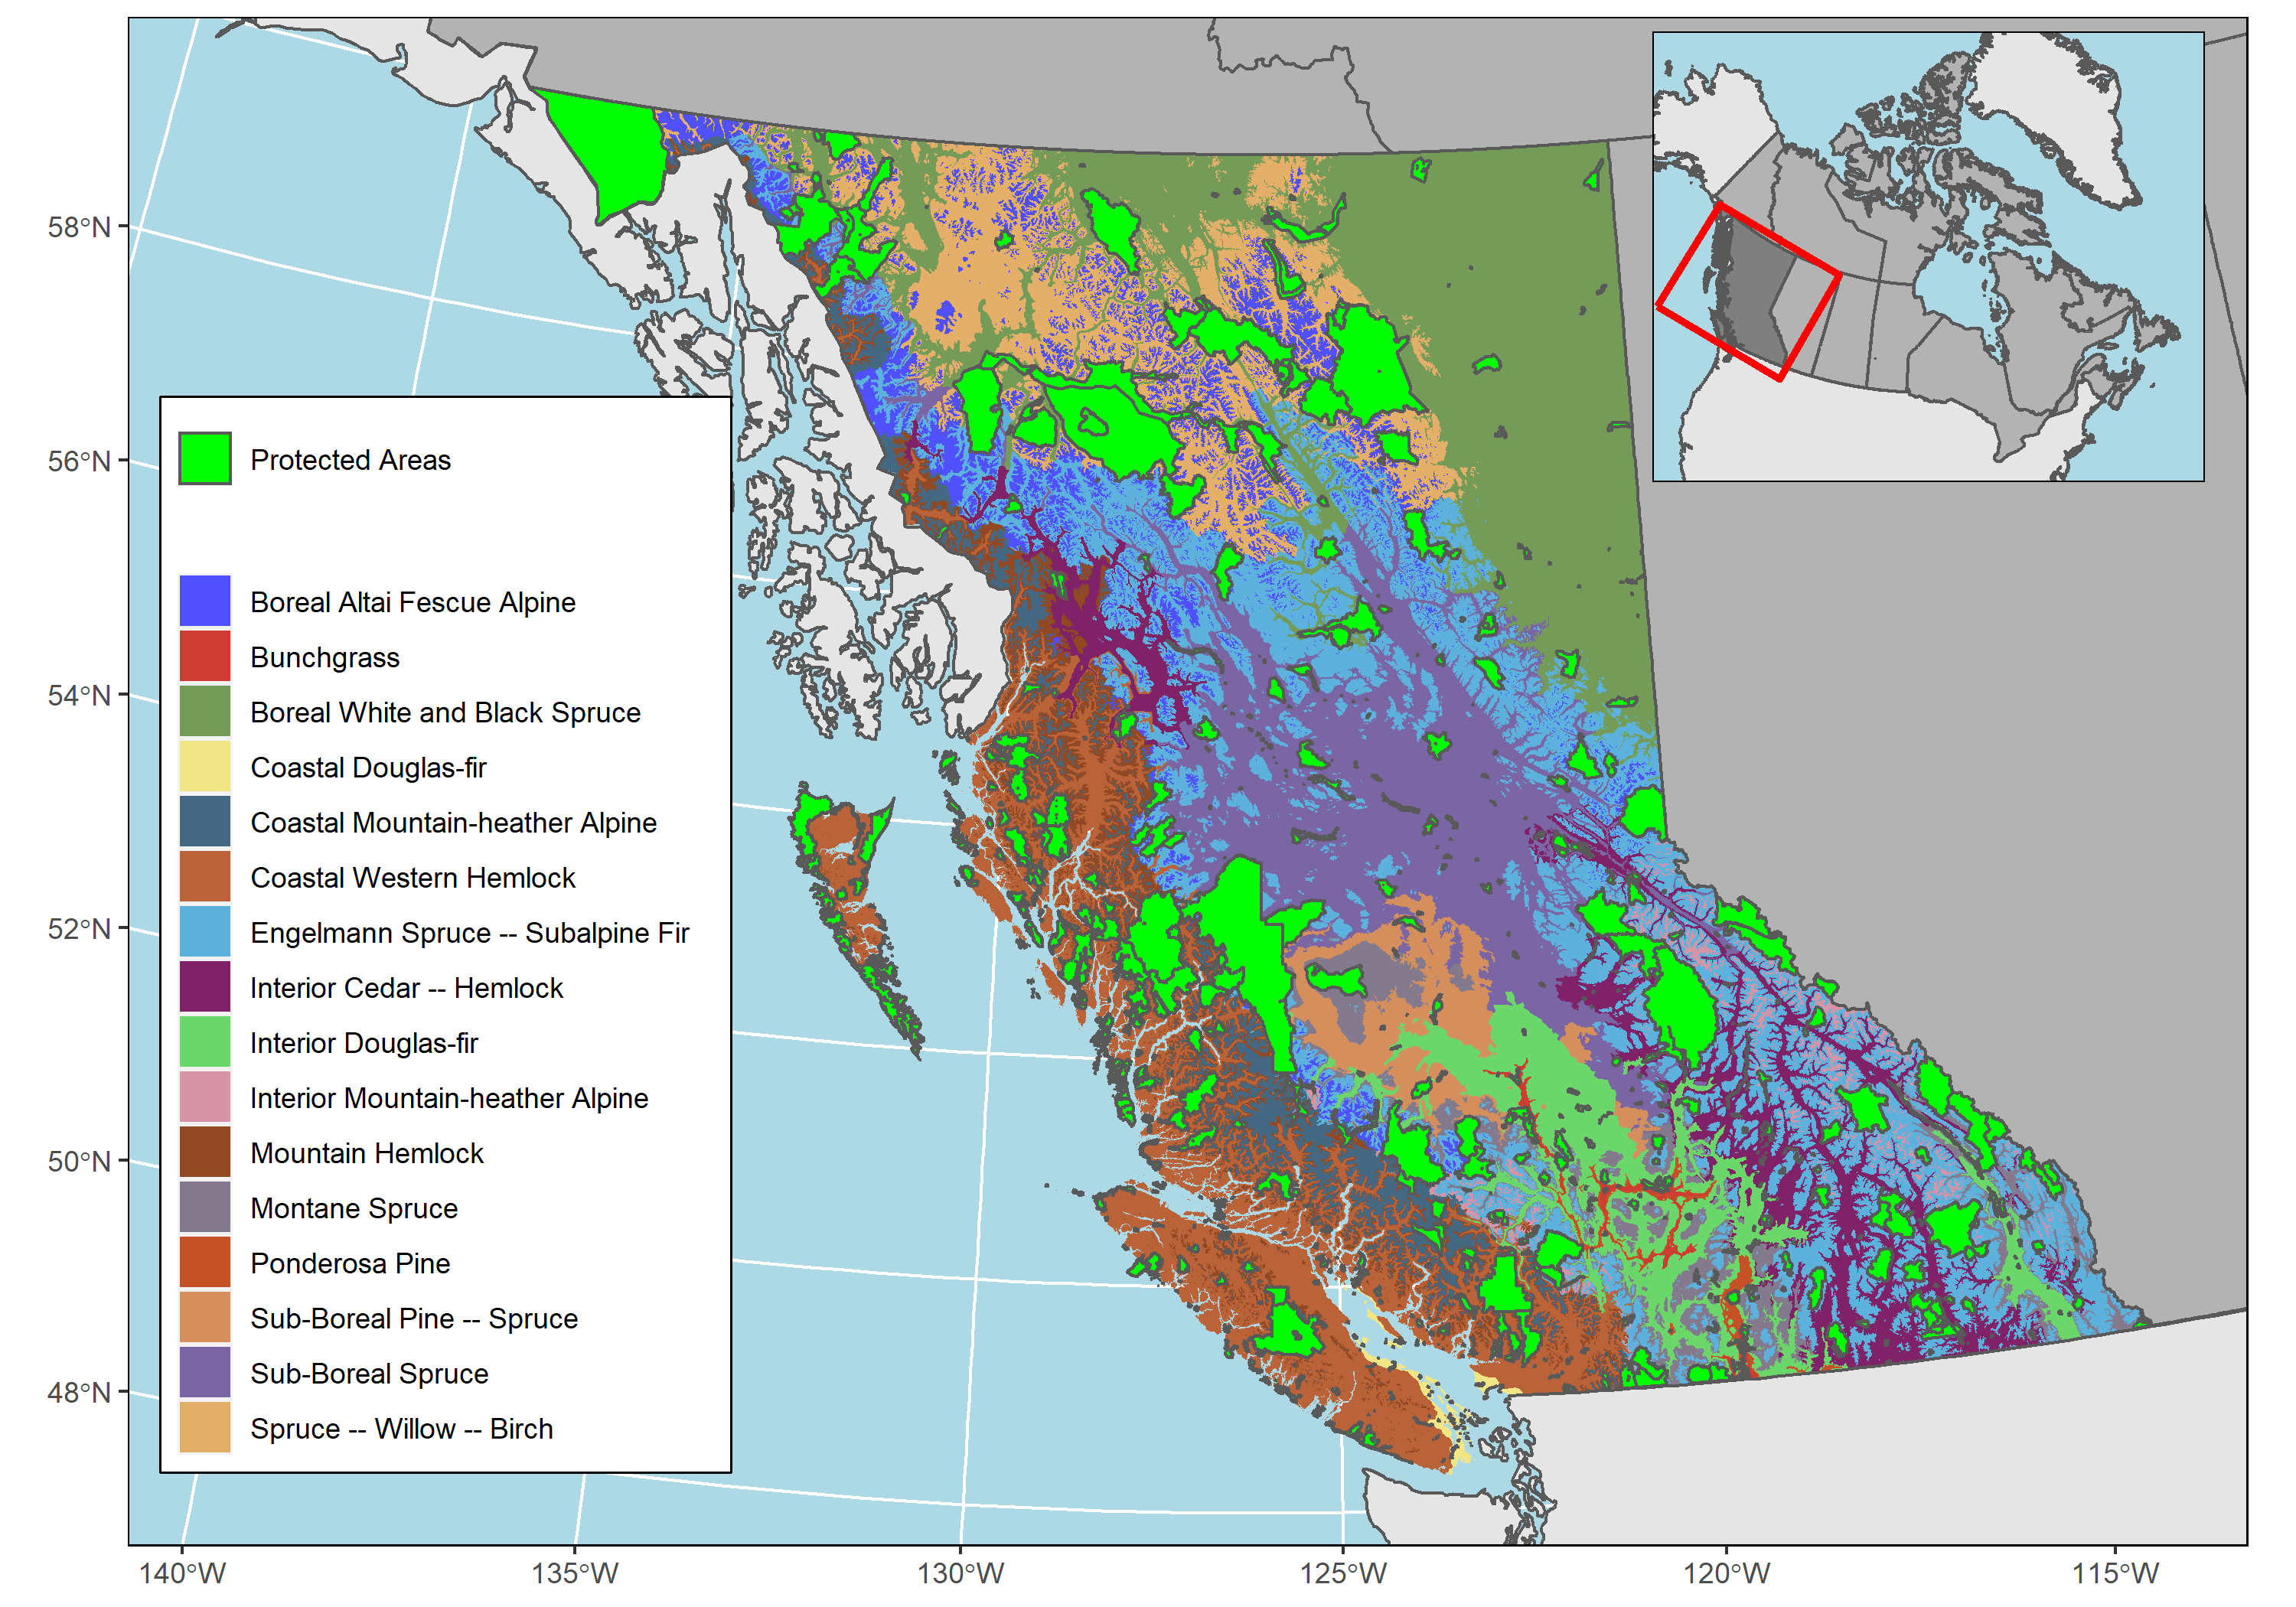
\includegraphics{figures/bec_map.png}
\caption{Terrestrial British Columbia including BEC zones and the
location of PA selected in this study.}\label{fig:study-area}
}
\end{figure}

\hypertarget{data}{%
\subsection{Data}\label{data}}

\hypertarget{biogeoclimatic-ecosystem-classification-and-protected-areas}{%
\subsubsection{Biogeoclimatic Ecosystem Classification and Protected
Areas}\label{biogeoclimatic-ecosystem-classification-and-protected-areas}}

Boundaries for BEC zones and subzones were acquired using the
\textbf{bcmaps} R package (Teucher et al. 2021). Two BEC subzones were
entirely subsumed by PA (Boreal White and Black Spruce - Very Wet Cool
and Spruce -- Willow -- Birch - Very Wet Cool Shrub), whereas the
Sub-Boreal Pine -- Spruce - Moist Cool subzone has no PA representation.

Boundaries for all PA in BC were obtained from the Canadian Protected
and Conserved Areas Database (available from
\url{https://cws-scf.ca/CPCAD-BDCAPC_Dec2020.gdb.zip}), current as of
December 2020, and includes the International Union for Conservation of
Nature (IUCN) classification for each PA. PA were selected for analysis
following the criteria outlined in Bolton et al. (2019). Only parks
which belonged to IUCN classes Ia, Ib, II, and IV were selected, as
these categories are considered strictly protected. Protected areas
\textless{} 100 ha in size were also excluded from the analysis, as
these mainly occurred in urbanized areas. After selection, 745 suitable
parks managed under various jurisdictions (provincial, federal, NGOs),
comprising 15.4\% of the total terrestrial area of British Columbia,
were studied (Environmental Reporting BC 2016). An equal sample of
pixels equal to the area of PA or UA - whichever was lower - was
randomly selected from both PA and UA for each BEC subzone. This
sampling regime accounts for bias in topography, climate, and climax
species due to the methods used to delineate BEC zones and subzones
(Pojar et al. 1987).

\hypertarget{digital-elevation-model}{%
\subsubsection{Digital Elevation Model}\label{digital-elevation-model}}

The Advanced Spaceborne Thermal Emission and Reflection Radiometer
(ASTER) digital elevation model (GDEM V2, 30 m) was used to examine
biases in protected area land cover and ecological classification by
elevation (Tachikawa et al. 2011).

\hypertarget{landsat-derived-datasets}{%
\subsubsection{Landsat derived
datasets}\label{landsat-derived-datasets}}

Land cover, forest disturbances, and forest structural attributes for BC
were derived from the annual Landsat best-available-pixel (BAP)
composites from 1984 to 2019 at 30-m spatial resolution generated using
the Composite2Change (C2C) approach (Hermosilla et al. 2016). These
composites are generated by annually selecting the optimal observations,
free from atmospheric effects (haze, clouds, cloud shadows), for each
pixel from the catalog of available Landsat-5 Thematic Mapper (TM),
Landsat-7 Enhanced Thematic Mapper Plus (ETM+), and Landsat-8
Operational Land Imager (OLI) imagery acquired during Canada's growing
season using the scoring functions defined in White et al. (2014). The
annual BAP composites are further refined by applying a spectral trend
analysis over the Normalized Burn Ratio (NBR) at pixel level in order to
remove unscreened noise, detect changes and fill data gaps with
temporally-interpolated values, resulting in annual, gap-free,
surface-reflectance image composites (Hermosilla et al. 2015b). During
this process, forest disturbances are detected, characterized and
attributed to a disturbance agent (i.e., wildfire, harvest, non-stand
replacing disturbances) using a Random Forests classification model via
the object-based analysis approach (Hermosilla et al. 2015a) with an
overall accuracy of 92\% ±2\% (Hermosilla et al. 2016).

Annual land cover information for Canada was produced using the BAP
composites following the Virtual Land Cover Engine framework (Hermosilla
et al. 2018). This framework integrates post-classification
probabilities, forest disturbance information and forest successional
knowledge with a Hidden Markov Model to ensure logical land cover
transitions between years. The classification comprises 12 land cover
classes organized as either non-vegetated or vegetated. Non-vegetated
classes included water, snow/ice, rock/rubble, and exposed/barren land.
Vegetated land cover classes discriminated among non-treed and treed
vegetation (land-cover level). Vegetated non-treed classes comprised
bryoids, herbs, wetland, and shrubs. Vegetated treed land cover classes
included wetland-treed, coniferous, broadleaf, and mixed wood.
Independent validation of the land cover maps indicated an overall
accuracy of 70.3\% ± 2.5\%.

Wall-to-wall, 30-m forest structure metrics (i.e., Lorey's height, total
aboveground biomass, elevation covariance, and canopy cover) were also
annually derived from the BAP composites using the imputation method
described in Matasci et al. (2018b, 2018a). This method uses lidar and
field plot data to estimate forest structure metrics from topographic
and Landsat spectral predictors, using a k-Nearest Neighbor approach.
Reported accuracy for the structure metrics indicated a RMSE\% ranging
from 24.5\% to 65.8\% and a R\textsuperscript{2} ranging from 0.125 to
0.699 (Matasci et al. 2018a).

Forest cover classes (deciduous, broadleaf, mixed-wood, and
wetland-treed) were used to generate land cover masks to restrict the
comparison of forest structural attributes to treed pixels. Pixels with
harvest activity disturbances detected post-1985 were also removed from
forest structural attribute rasters in both PA and UA, in order to
restrict analysis to non-anthropogenically disturbed areas. All datasets
are displayed in fig.~\ref{fig:data-fig}.

\begin{figure}
\hypertarget{fig:data-fig}{%
\centering
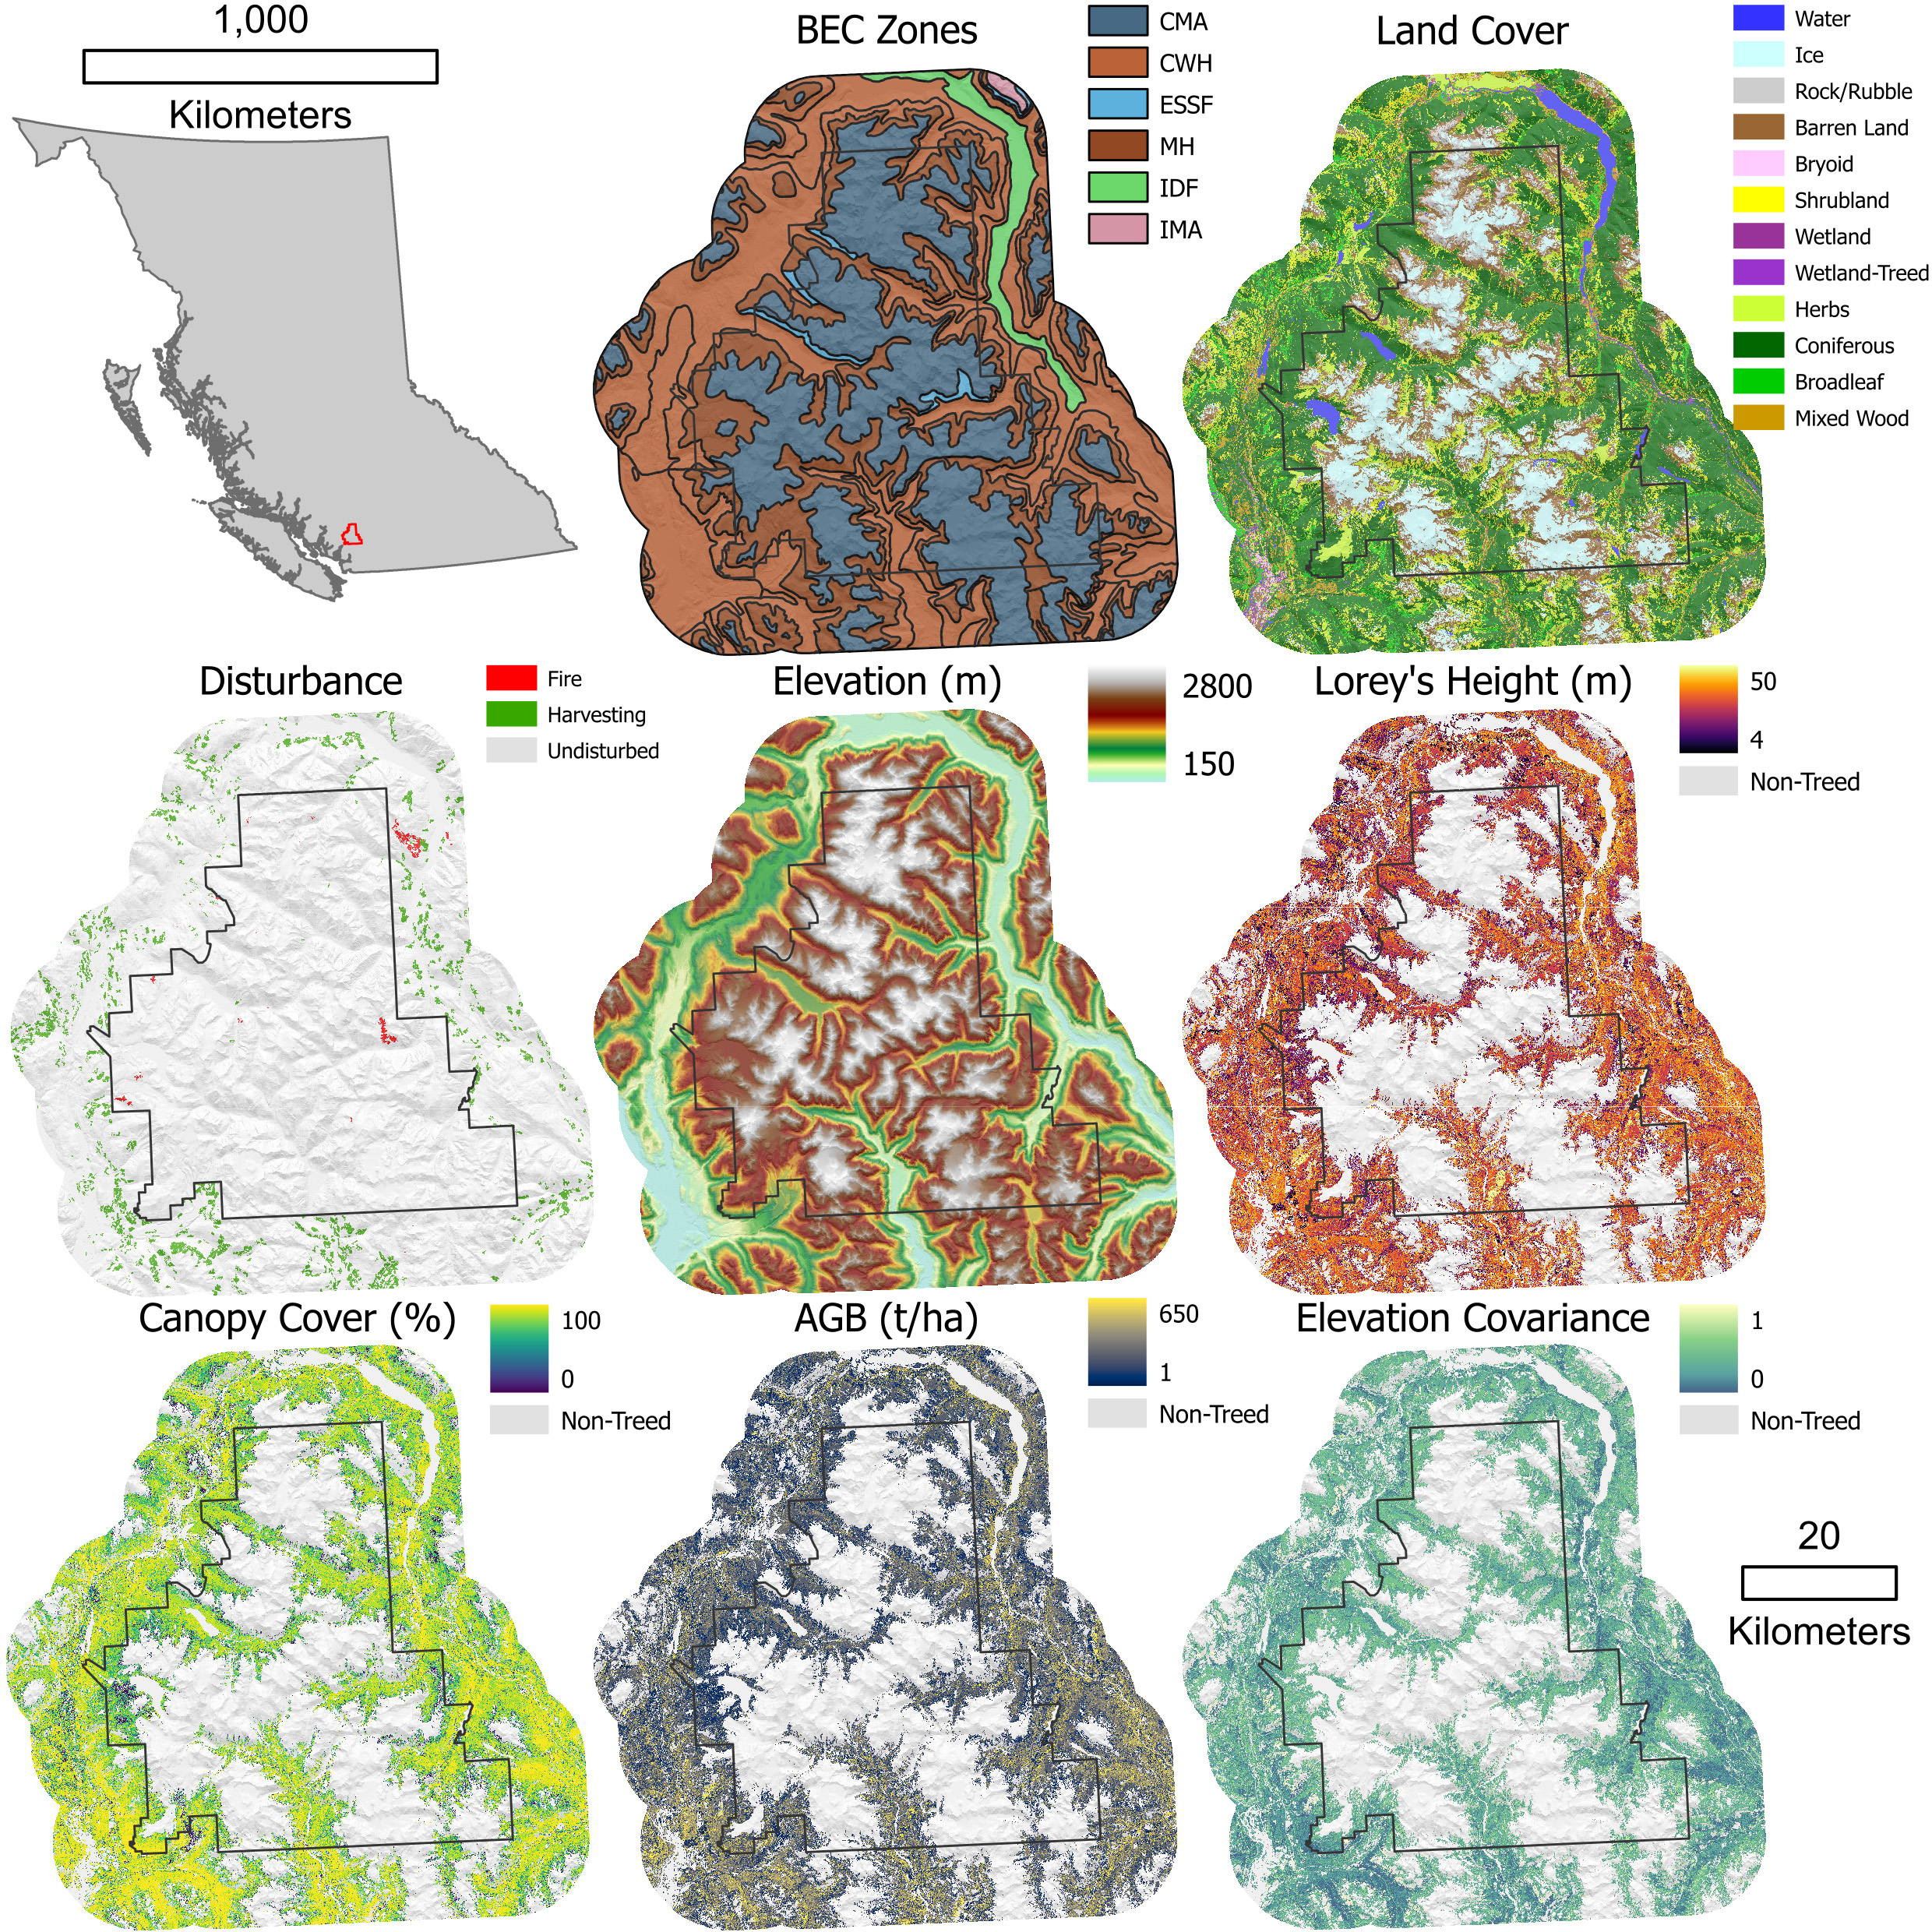
\includegraphics{figures/data_map.png}
\caption{Visualizations for all layers included in the analysis for
Garibaldi Park and surrounding region (red outline) in BC for
2015.}\label{fig:data-fig}
}
\end{figure}

\hypertarget{analysis}{%
\subsection{Analysis}\label{analysis}}

To determine bias in ecosystem representation in BC's PA network, we
compared BEC zone, land cover, and disturbance proportions within and
outside the PA network. We employ counterfactual thinking by examining
BEC zone, and land cover as a function of elevation, and secondly
compiled disturbance rates on a latitudinal gradient across the
province. Forest structural attributes were then examined at a finer
ecosystem classification level, statistically comparing PA vs UA across
similar ecosystems. Forest structural means across BC zones were
calculated to determine which forest structures need additional
representation in the current BC PA network. All data manipulation and
analysis was conducted in the \textbf{R} (R Core Team 2021) or
\textbf{Python} programming languages.

\hypertarget{ecosystems-land-cover-and-disturbances}{%
\subsubsection{Ecosystems, Land Cover, and
Disturbances}\label{ecosystems-land-cover-and-disturbances}}

BEC zones and land cover classifications were aggregated to both PA and
UA in order to determine the proportion of each zone under the protected
classifications, to examine progress towards the Aichi biodiversity
targets. In this analysis, zones were used to examine categorical data
(land cover and disturbance) for the period of 1984-2019. Land cover and
BEC zones were further examined along an elevation gradient, at 50m
increments. Histograms of area by elevation were generated in order to
examine the areal magnitude alongside the proportional coverage of land
cover and BEC zones. This allows us to examine the amount of area
protected at each elevation, as well as the differences between PA and
UA. Forest disturbances (including harvesting) were aggregated along a
latitudinal gradient at increments of 0.5°.

\hypertarget{forest-structural-attributes}{%
\subsubsection{Forest Structural
Attributes}\label{forest-structural-attributes}}

T-tests for PA vs UA were conducted on all pixels selected for analysis
by BEC subzone and forest structural attribute for 2015, and the
Bonferroni correction was applied. The Bonferroni correction avoids
spuriously significant results in multiple comparison tests by dividing
the significant p-value (0.01) by the number of tests (Bonferroni 1936).
Within each BEC zone, higher proportions of significant tests will
indicate dissimilar subzones in each forest structural attribute. The
mean values for PA and UA forest structural attributes were calculated,
in order to examine the differences in their distribution and determine
which structures and zones differ between PA and UA. Values were also
converted into z-scores to determine the greatest standardized vector
magnitude when comparing canopy cover, elevation covariance, and forest
height between PA and UA.

\hypertarget{results}{%
\section{Results}\label{results}}

\hypertarget{ecosystems-land-cover-and-disturbances-1}{%
\subsubsection{Ecosystems, Land Cover, and
Disturbances}\label{ecosystems-land-cover-and-disturbances-1}}

British Columbia's ecosystems are protected at varying rates across the
province (fig.~\ref{fig:bec-conch}). Of the 16 ecosystems present in BC,
seven are protected at rates above the Aichi biodiversity target (17\%).
Only two zones (Boreal Altai Fescue Alpine and Interior Mountain-heather
Alpine) are currently protected at rates above the Canadian 2025
protection targets (25\%). Zones with Douglas-fir (\emph{Pseudotsuga
menziesii}) as dominant old-growth components (Coastal Douglas-fir and
Interior Douglas-fir) are the least proportionally represented zones in
British Columbia, with 4.9\% and 6.4\% protected, respectively
(fig.~\ref{fig:bec-conch}).

\begin{figure}
\hypertarget{fig:bec-conch}{%
\centering
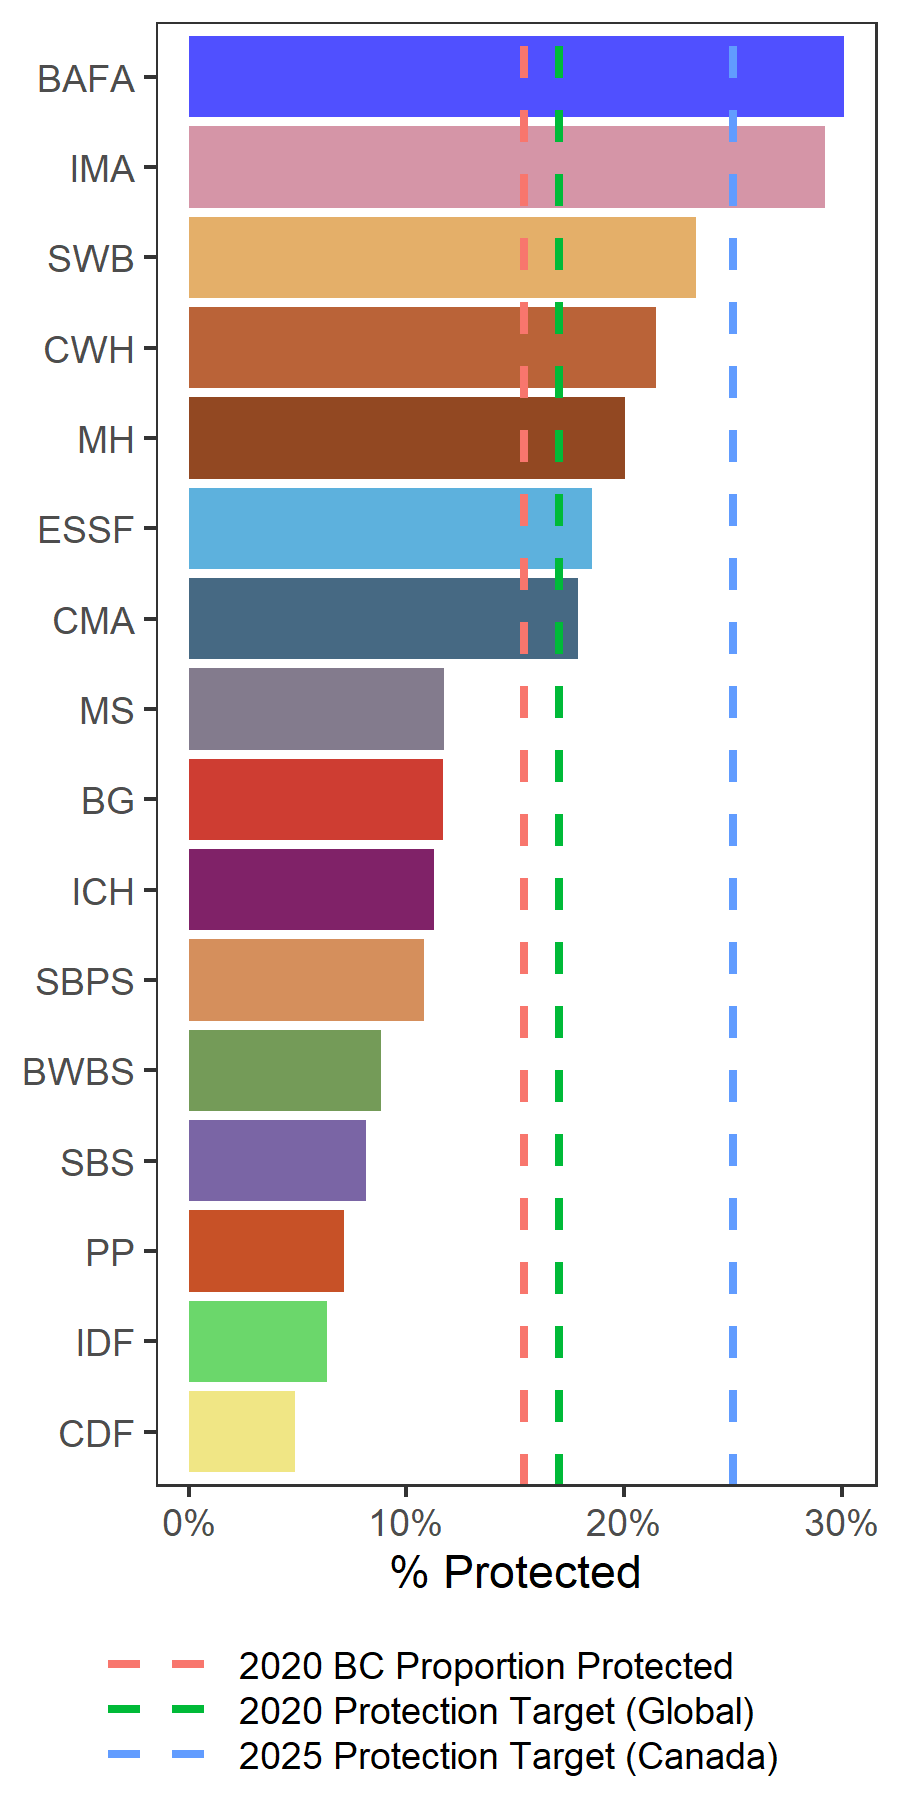
\includegraphics{figures/bec_bar.png}
\caption{Areal proportion of biogeoclimatic ecosystem classification
(BEC) zones protected in British Columbia (See Table 1 for full BEC zone
names).}\label{fig:bec-conch}
}
\end{figure}

As elevation increases in BC, increasing terrestrial area is protected
within the PA network until \textasciitilde4000m, upon which all
terrestrial area is protected (fig.~\ref{fig:bec-elev}). When comparing
between PA and UA, zones are protected at differing proportions. Zones
commonly found at high elevations, such as the Boreal Altai Fescue
Alpine, are predominantly located in protected areas, however, little
terrestrial area is found at these elevations. In low elevations,
proportions of area protected also differ, with Coastal Western Hemlock
having a large proportion of coverage in PA, while in UA, Boreal Black
and White Spruce are underrepresented. Generally, the remaining
ecosystems are found at similar rates in both PA and UA
(fig.~\ref{fig:bec-elev}).

\begin{figure}
\hypertarget{fig:bec-elev}{%
\centering
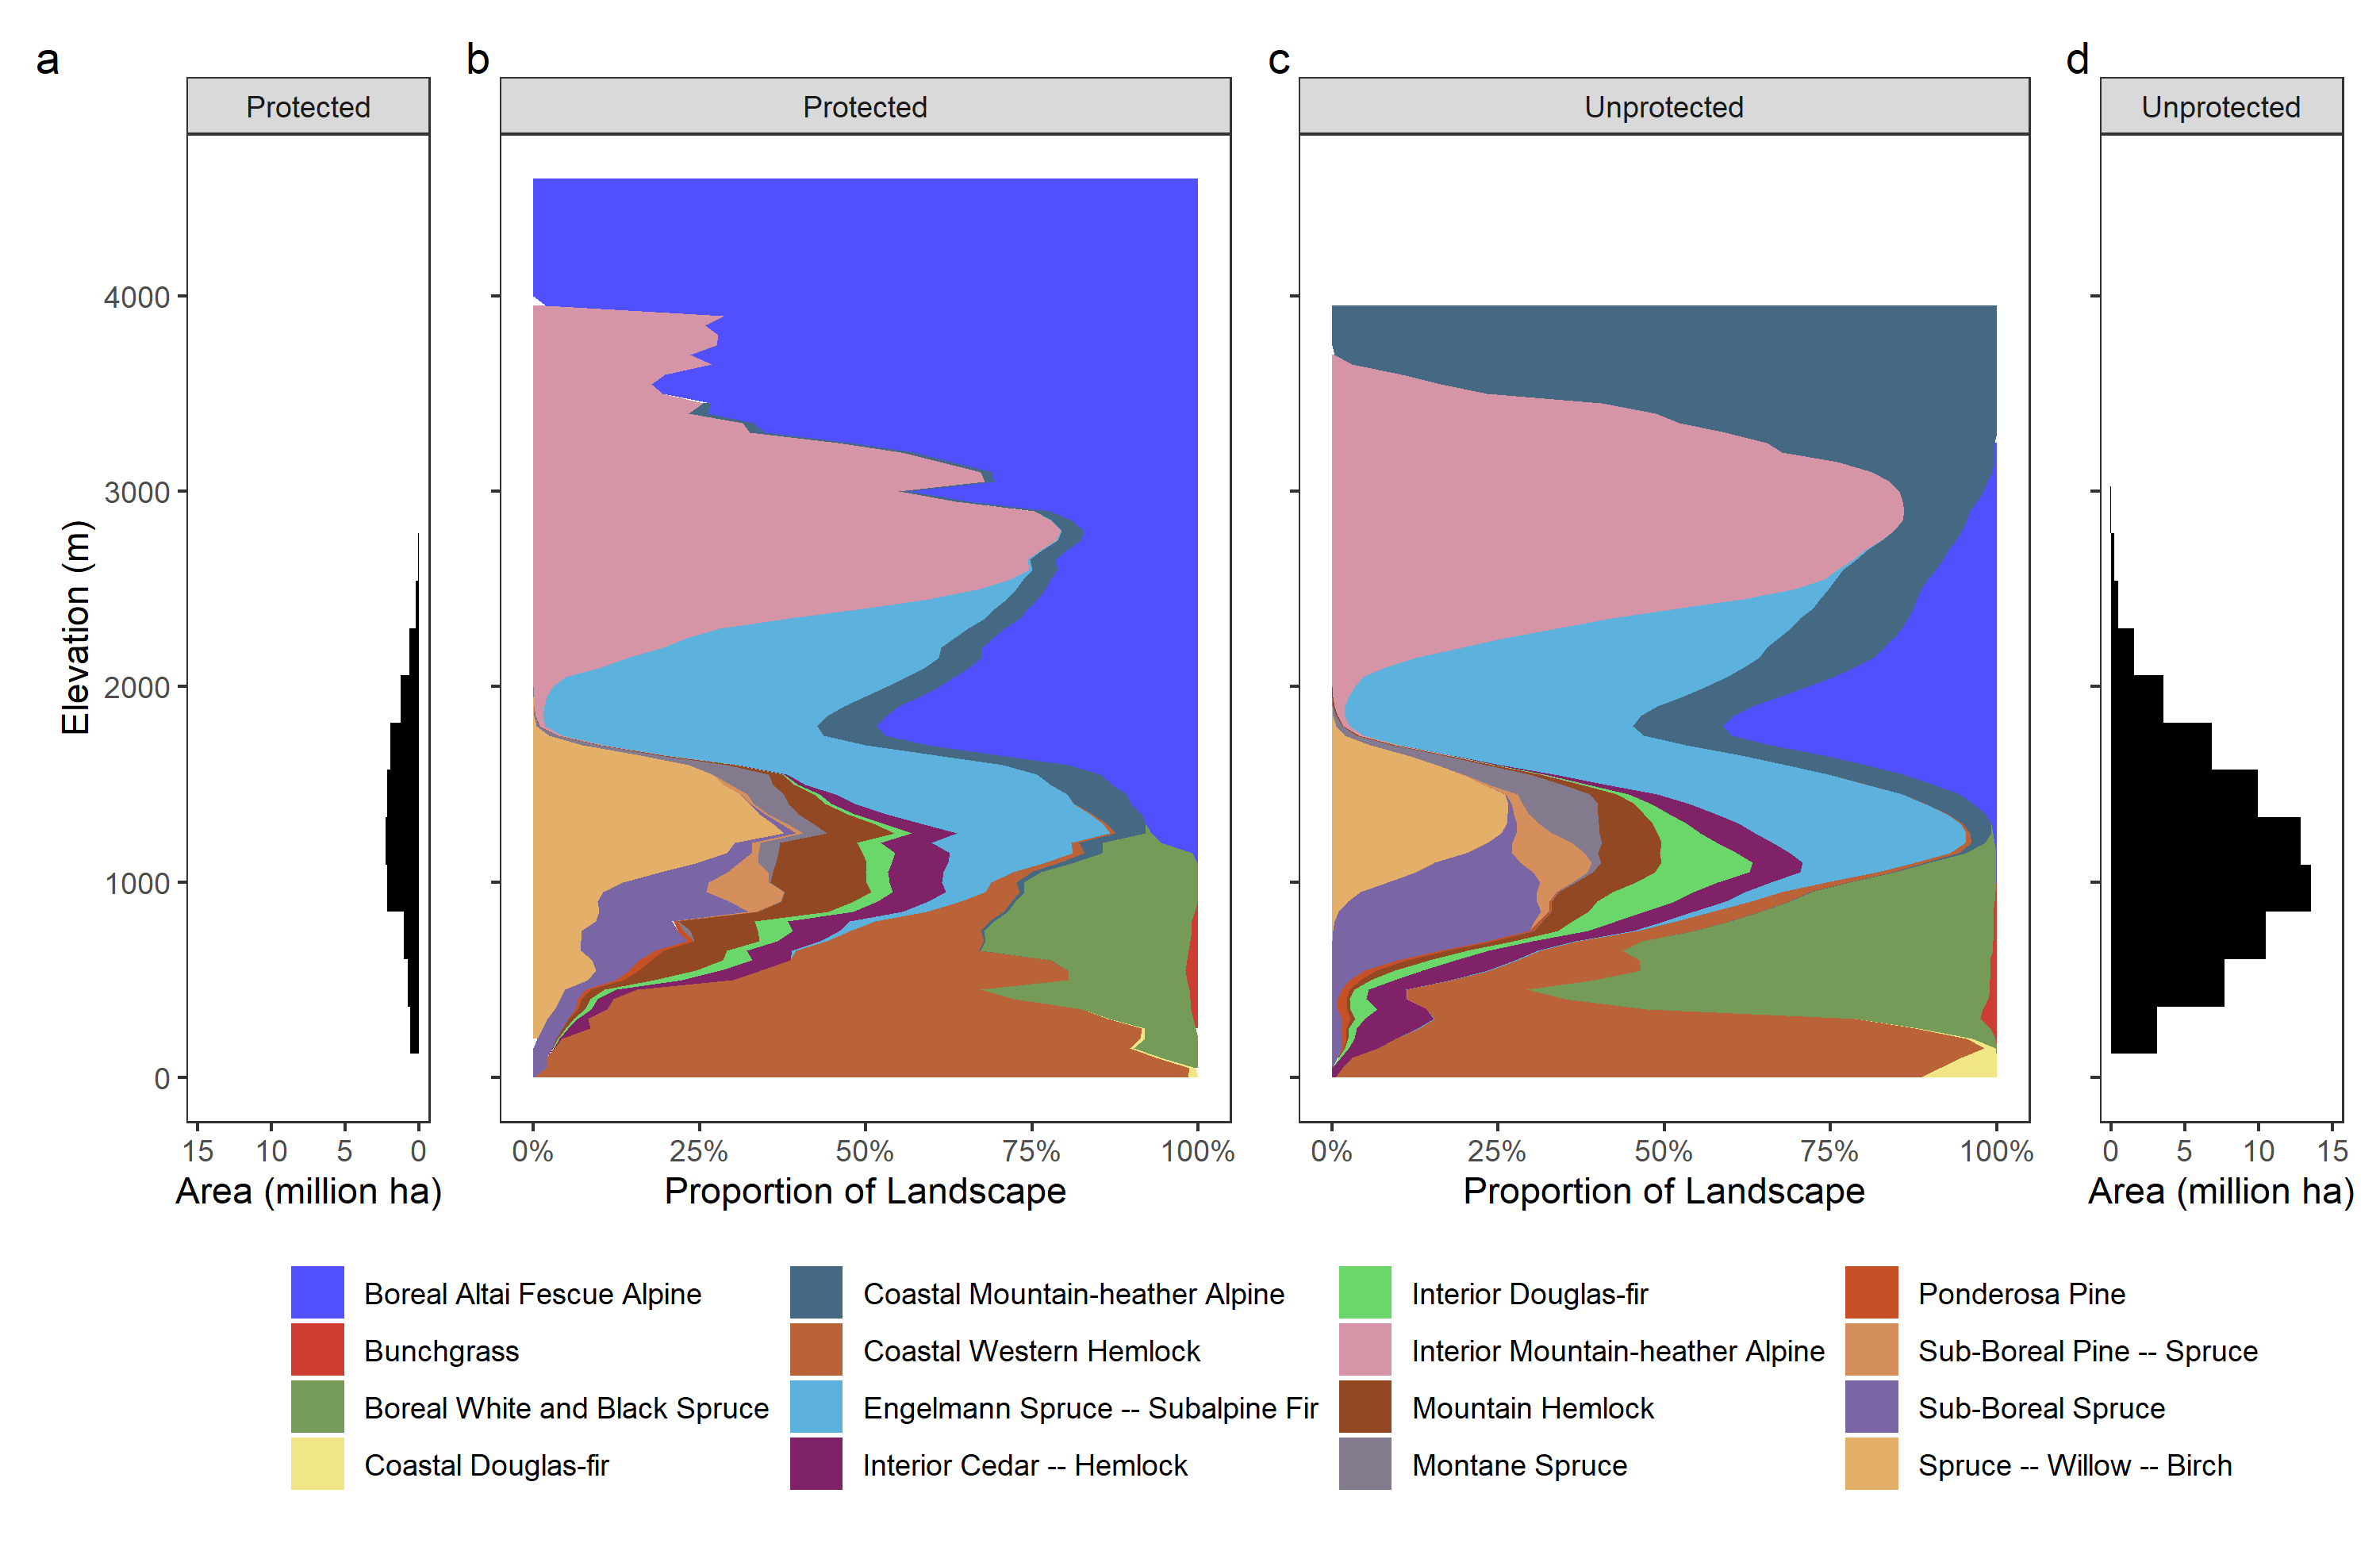
\includegraphics{figures/bec_elev_hist.png}
\caption{Histogram of area protected in British Columbia by Elevation
(a). Proportion of Biogeoclimatic Ecosystem Classification (BEC) zone by
elevation for both protected areas (b), and unprotected areas (c).
Histogram of area unprotected in British Columbia by Elevation
(d).}\label{fig:bec-elev}
}
\end{figure}

Protected land cover also varies by proportion
(fig.~\ref{fig:vlce-conch}). Non-vegetated classes of snow/ice,
exposed/barren land, and rock/rubble have higher than average
proportions protected while mixed wood and broadleaf land cover classes
are underrepresented. All other classes are found at rates similar to
the overall proportion of the province protected (\textasciitilde15\%;
fig.~\ref{fig:vlce-conch}).

\begin{figure}
\hypertarget{fig:vlce-conch}{%
\centering
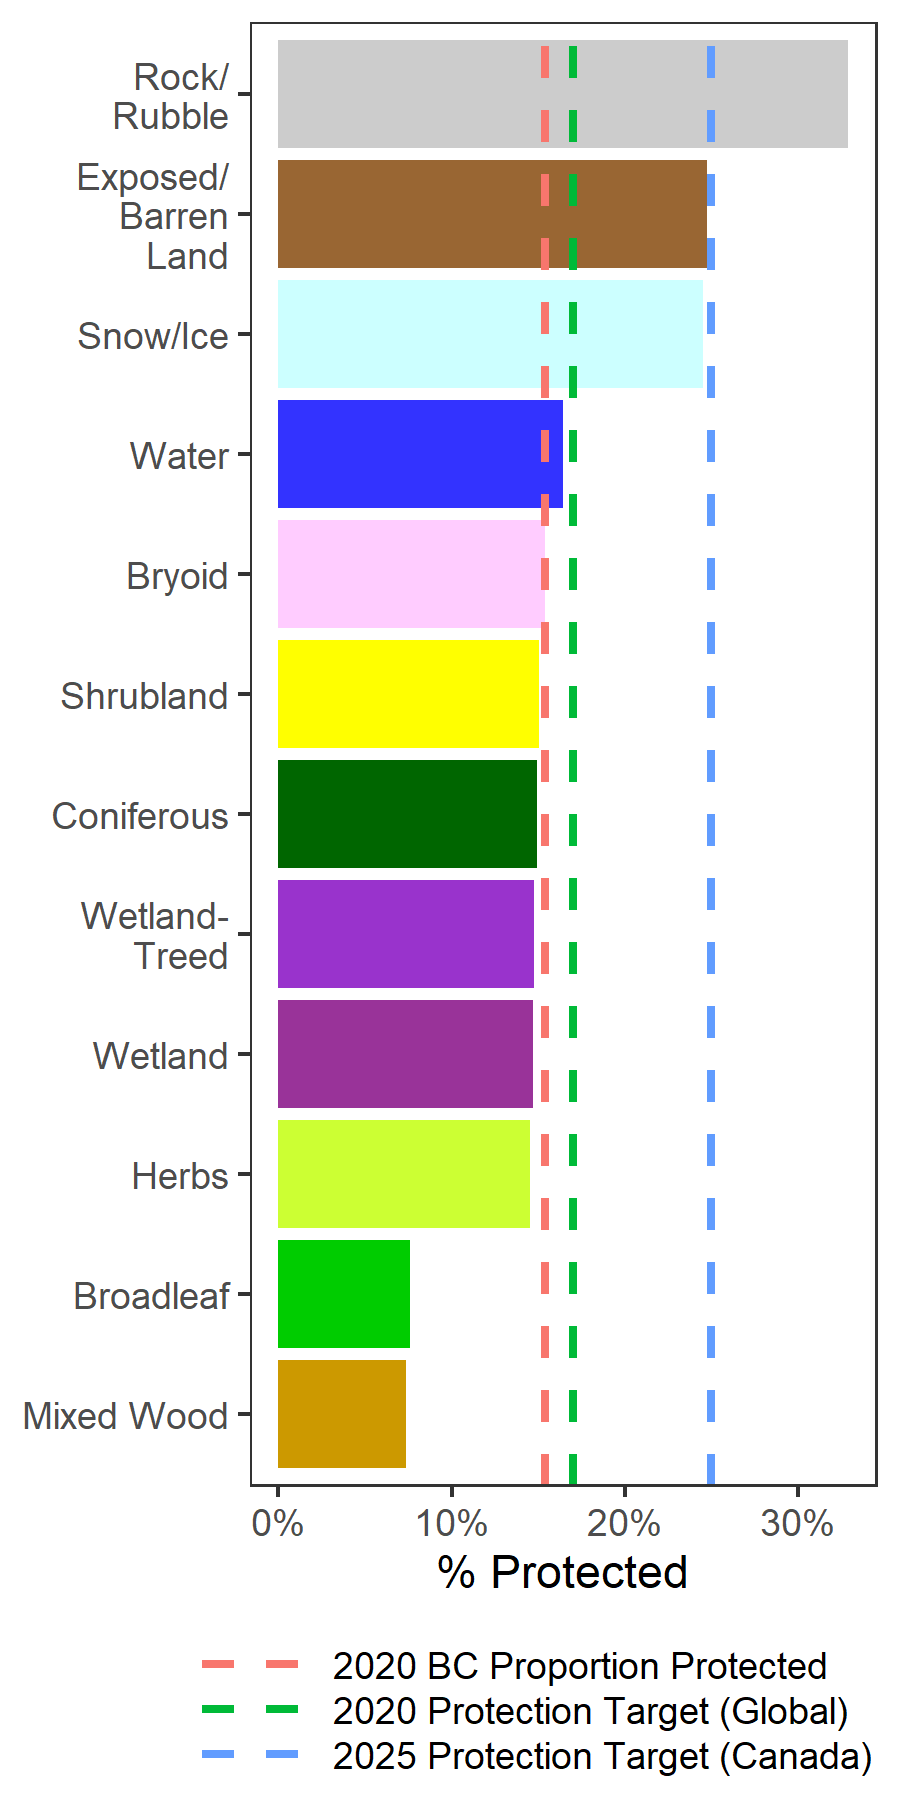
\includegraphics{figures/vlce_bar.png}
\caption{Areal proportion of land cover classes protected in
BC.}\label{fig:vlce-conch}
}
\end{figure}

Similar to BEC zones (fig.~\ref{fig:bec-elev}), land cover also varies
with elevation (fig.~\ref{fig:lcc-elev}). Expectedly, snow/ice make up a
large proportion of PA at higher elevations. At lower elevations in UA,
mixed wood forest is a more common forest type than in PA, while wetland
classes (wetland, wetland-treed) are less frequent in the 400-900m
elevation range in UA compared to PA.

\begin{figure}
\hypertarget{fig:lcc-elev}{%
\centering
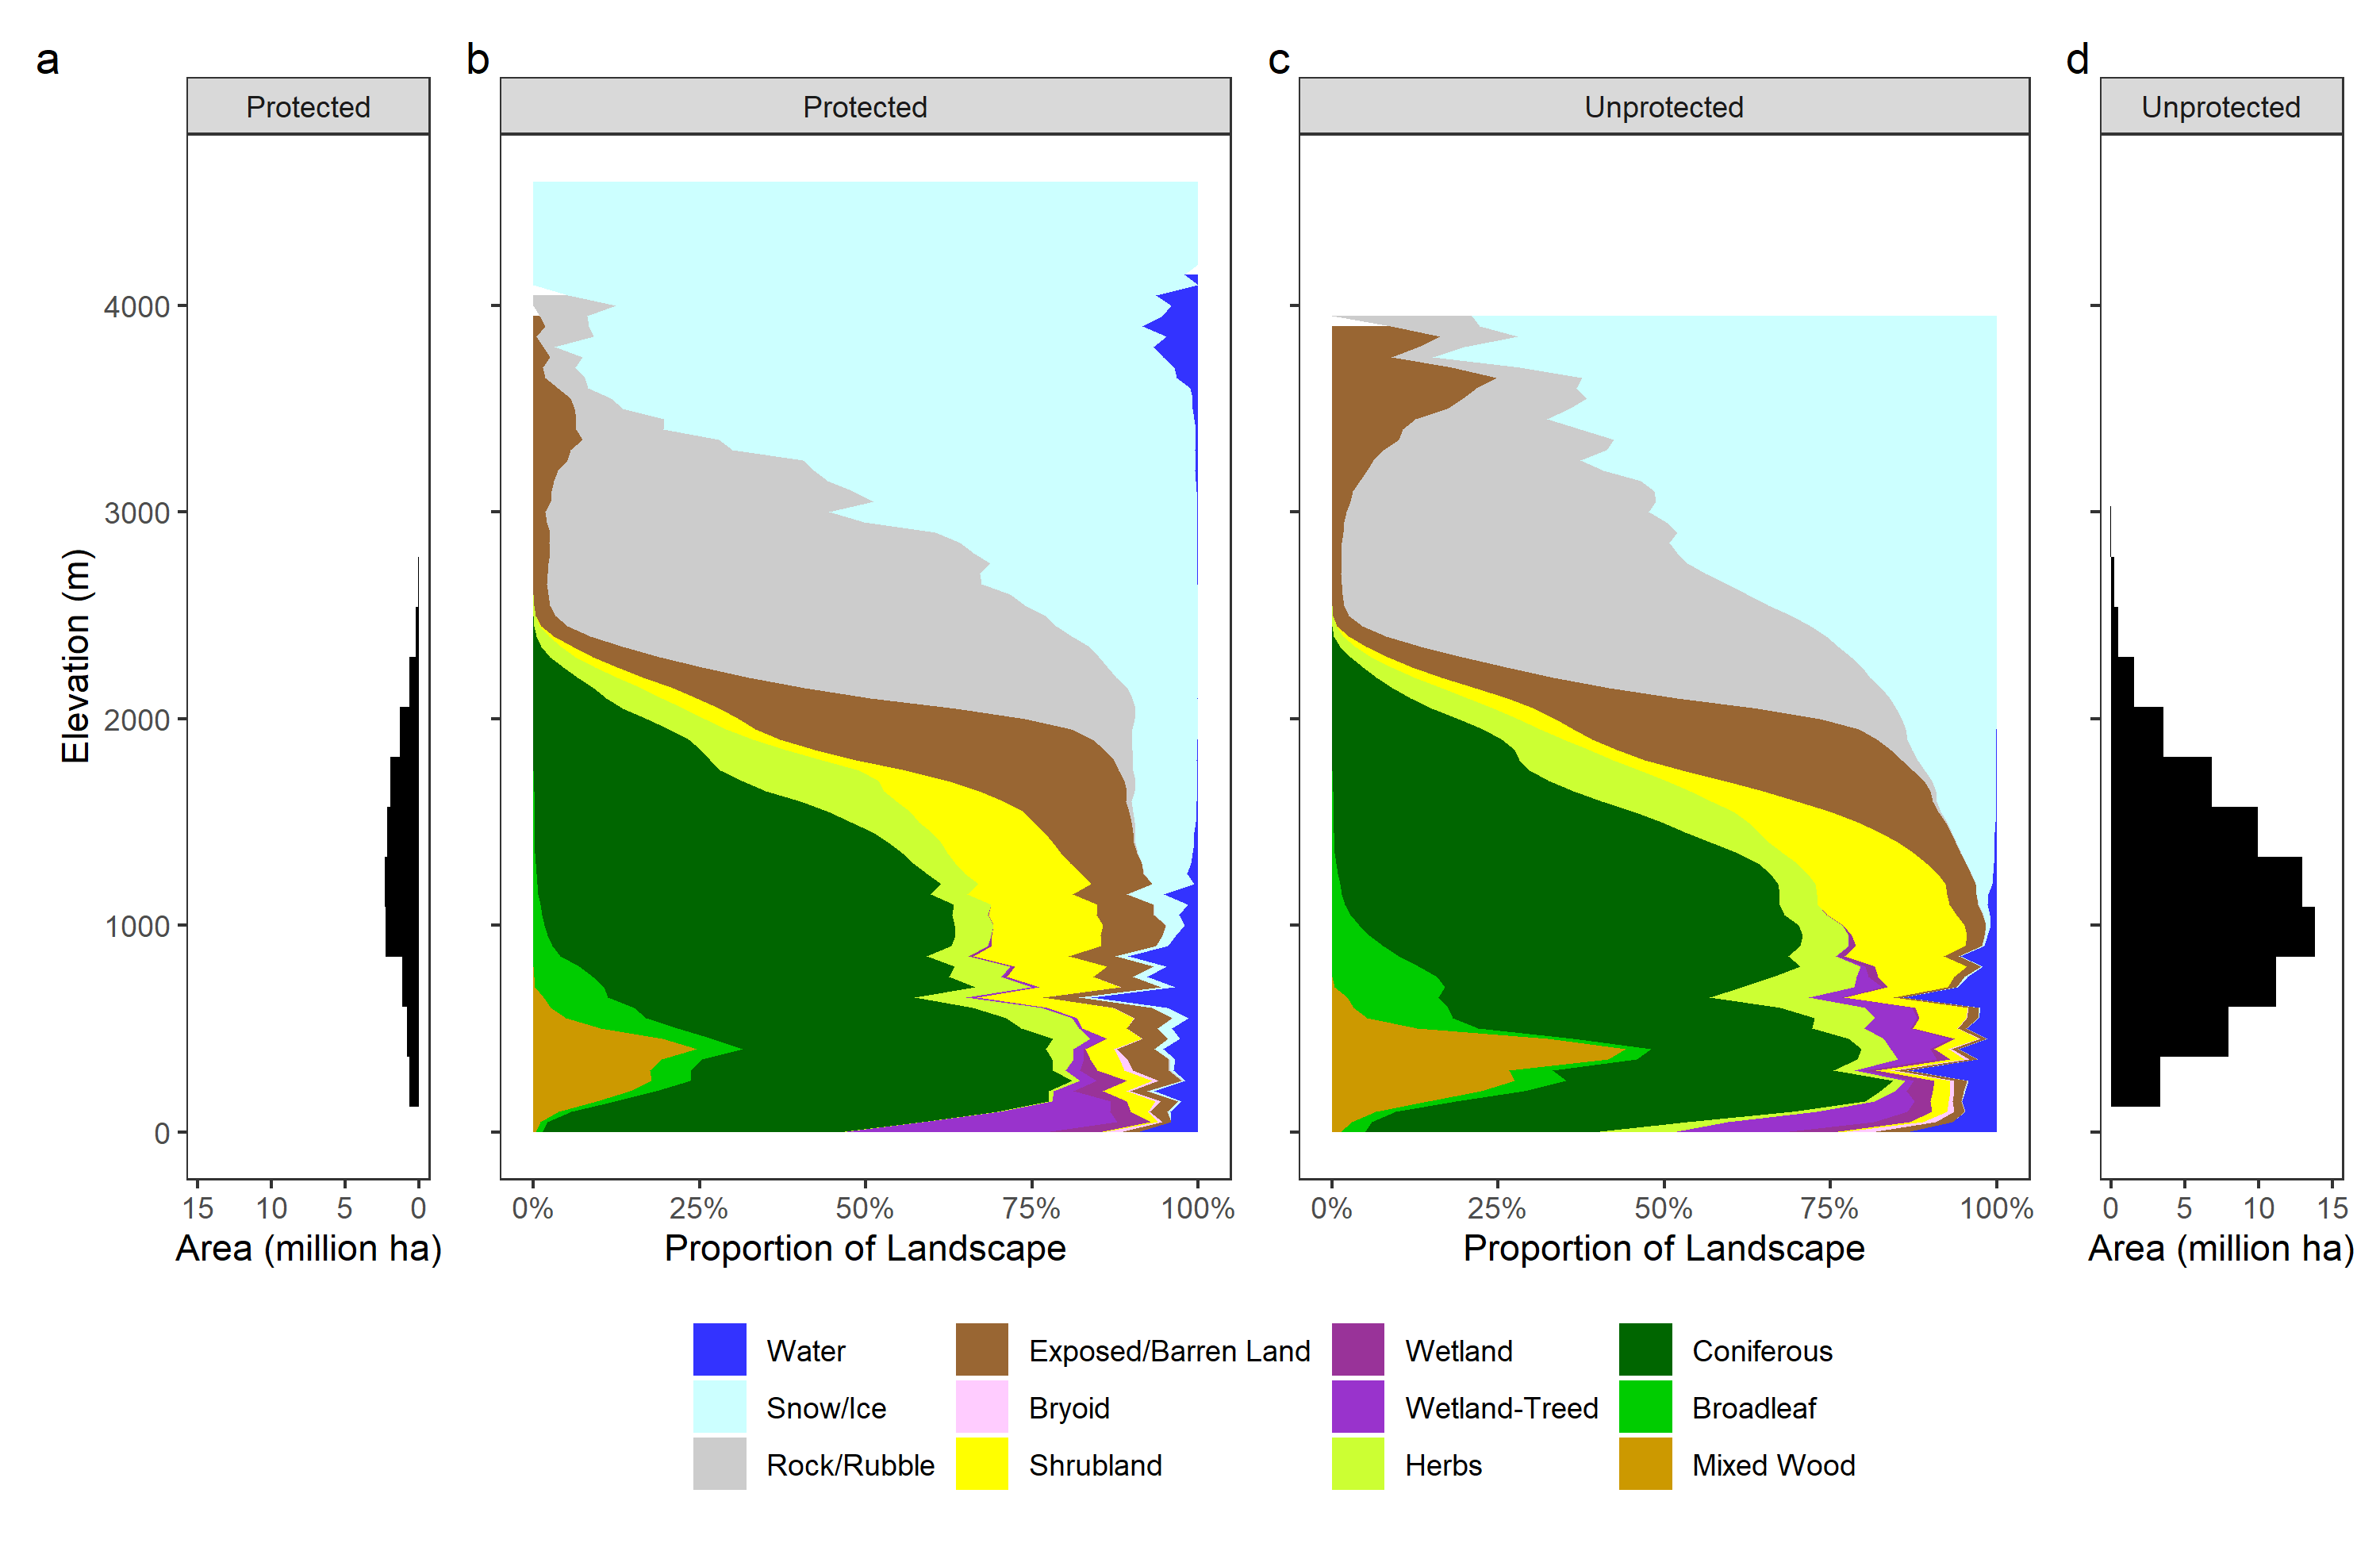
\includegraphics{figures/lcc_elev_hist.png}
\caption{Histogram of area protected in British Columbia by Elevation
(a) Proportion of land cover by elevation for both protected areas (b),
and unprotected areas (c). Histogram of area unprotected in British
Columbia by Elevation (d).}\label{fig:lcc-elev}
}
\end{figure}

Examining the elevation distributions of BEC zones and land cover
classes shows elevation variation in some classes and ecosystems
(fig.~\ref{fig:elev-boxplots}). Generally, BEC zones are found at
similar elevation profiles in both PA and UA. Alpine BEC zones (Interior
Mountain-heather Alpine, Boreal Altai Fescue Alpine, and Coastal
Mountain-heather Alpine) are found at similar elevations across PA and
UA, while other zones such as Sub-Boreal Pine -- Spruce, Ponderosa Pine,
and Bunchgrass vary in their elevation profiles. Land cover classes show
differences in the wetland, wetland-treed, and mixed wood classes. The
wetland classes are found at lower elevations in PA than UA, while the
mixed wood class has more variation in PA.

\begin{figure}
\hypertarget{fig:elev-boxplots}{%
\centering
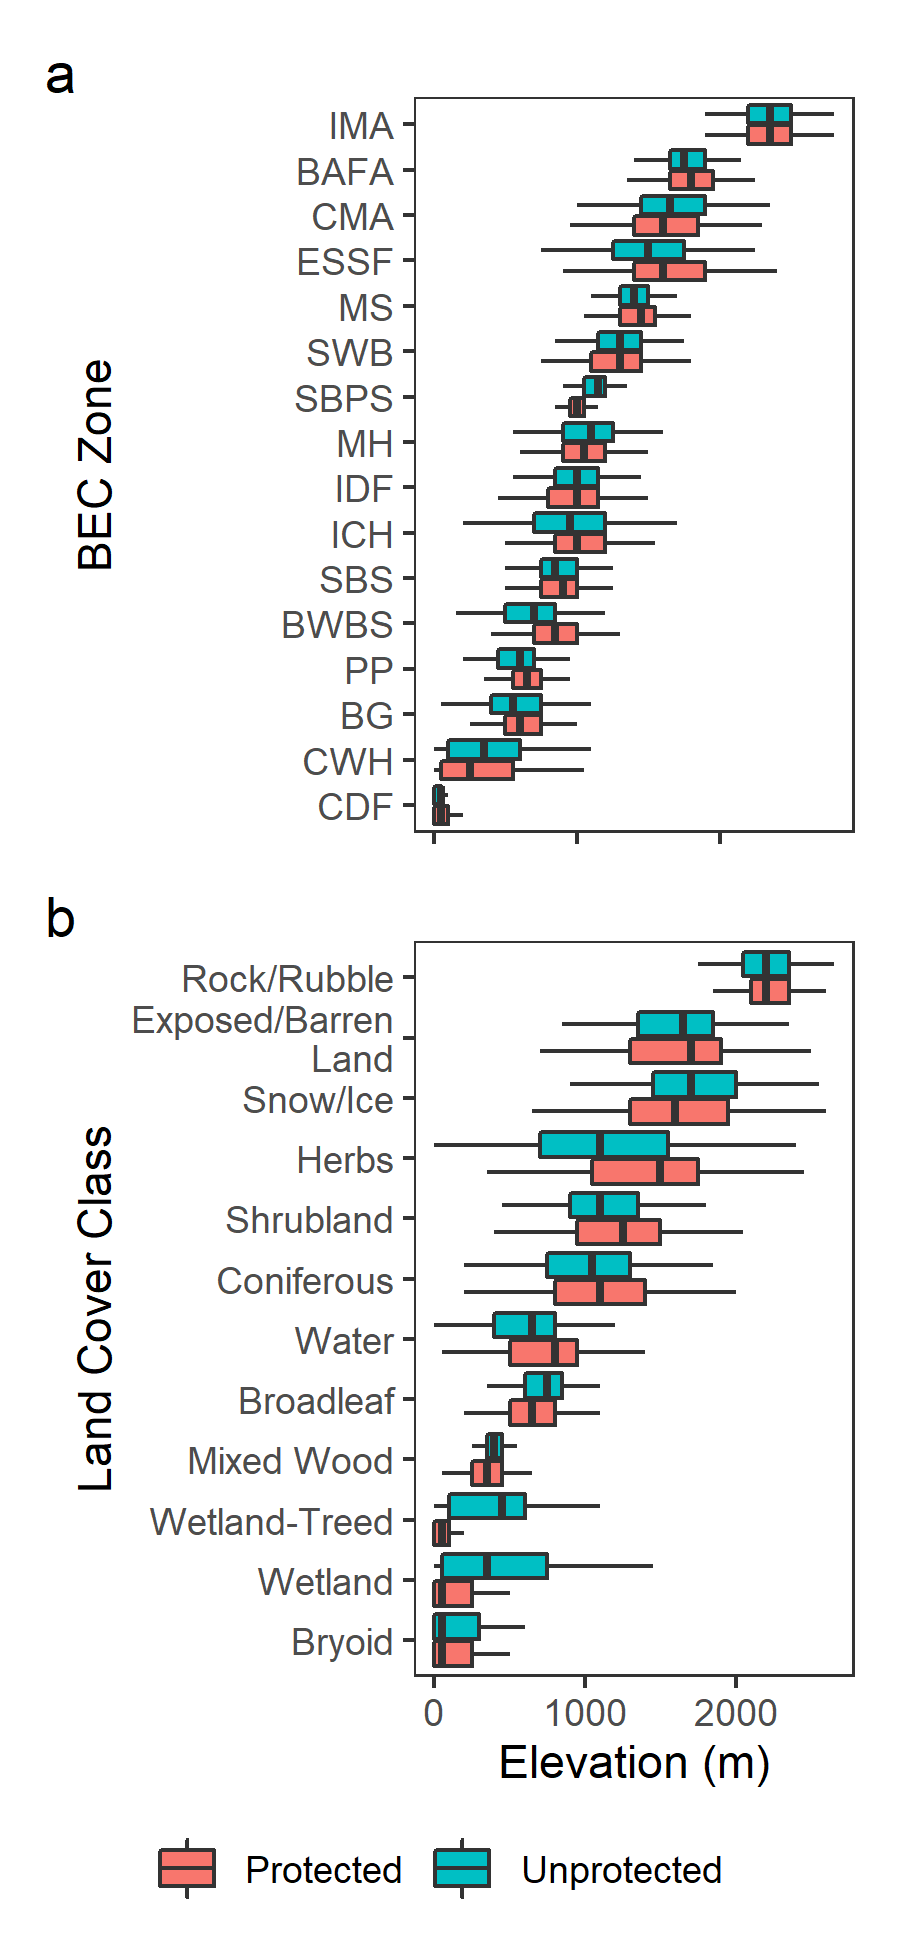
\includegraphics{figures/elev_boxplots.png}
\caption{Elevation boxplots for BEC zones (a), and land cover classes
(b). Whiskers indicate first quartile minus the interquartile range and
third quartile to the interquartile range. Box and interior vertical
line indicate first quartile, median, and third quartile,
respectively.}\label{fig:elev-boxplots}
}
\end{figure}

Overall, the burned area of forested cells is similar between PA (2.5\%
overall) and UA (2.3\%), while harvesting is much higher in UA (7.2\%)
than in PA (0.33\%). Harvesting is more common at lower latitudes in UA
than at higher latitudes. Fire shows similar, but not identical patterns
across varying latitudes, with higher wildfire proportions at high
latitudes and between 51-53°N (fig.~\ref{fig:lat-dist}).

\begin{figure}
\hypertarget{fig:lat-dist}{%
\centering
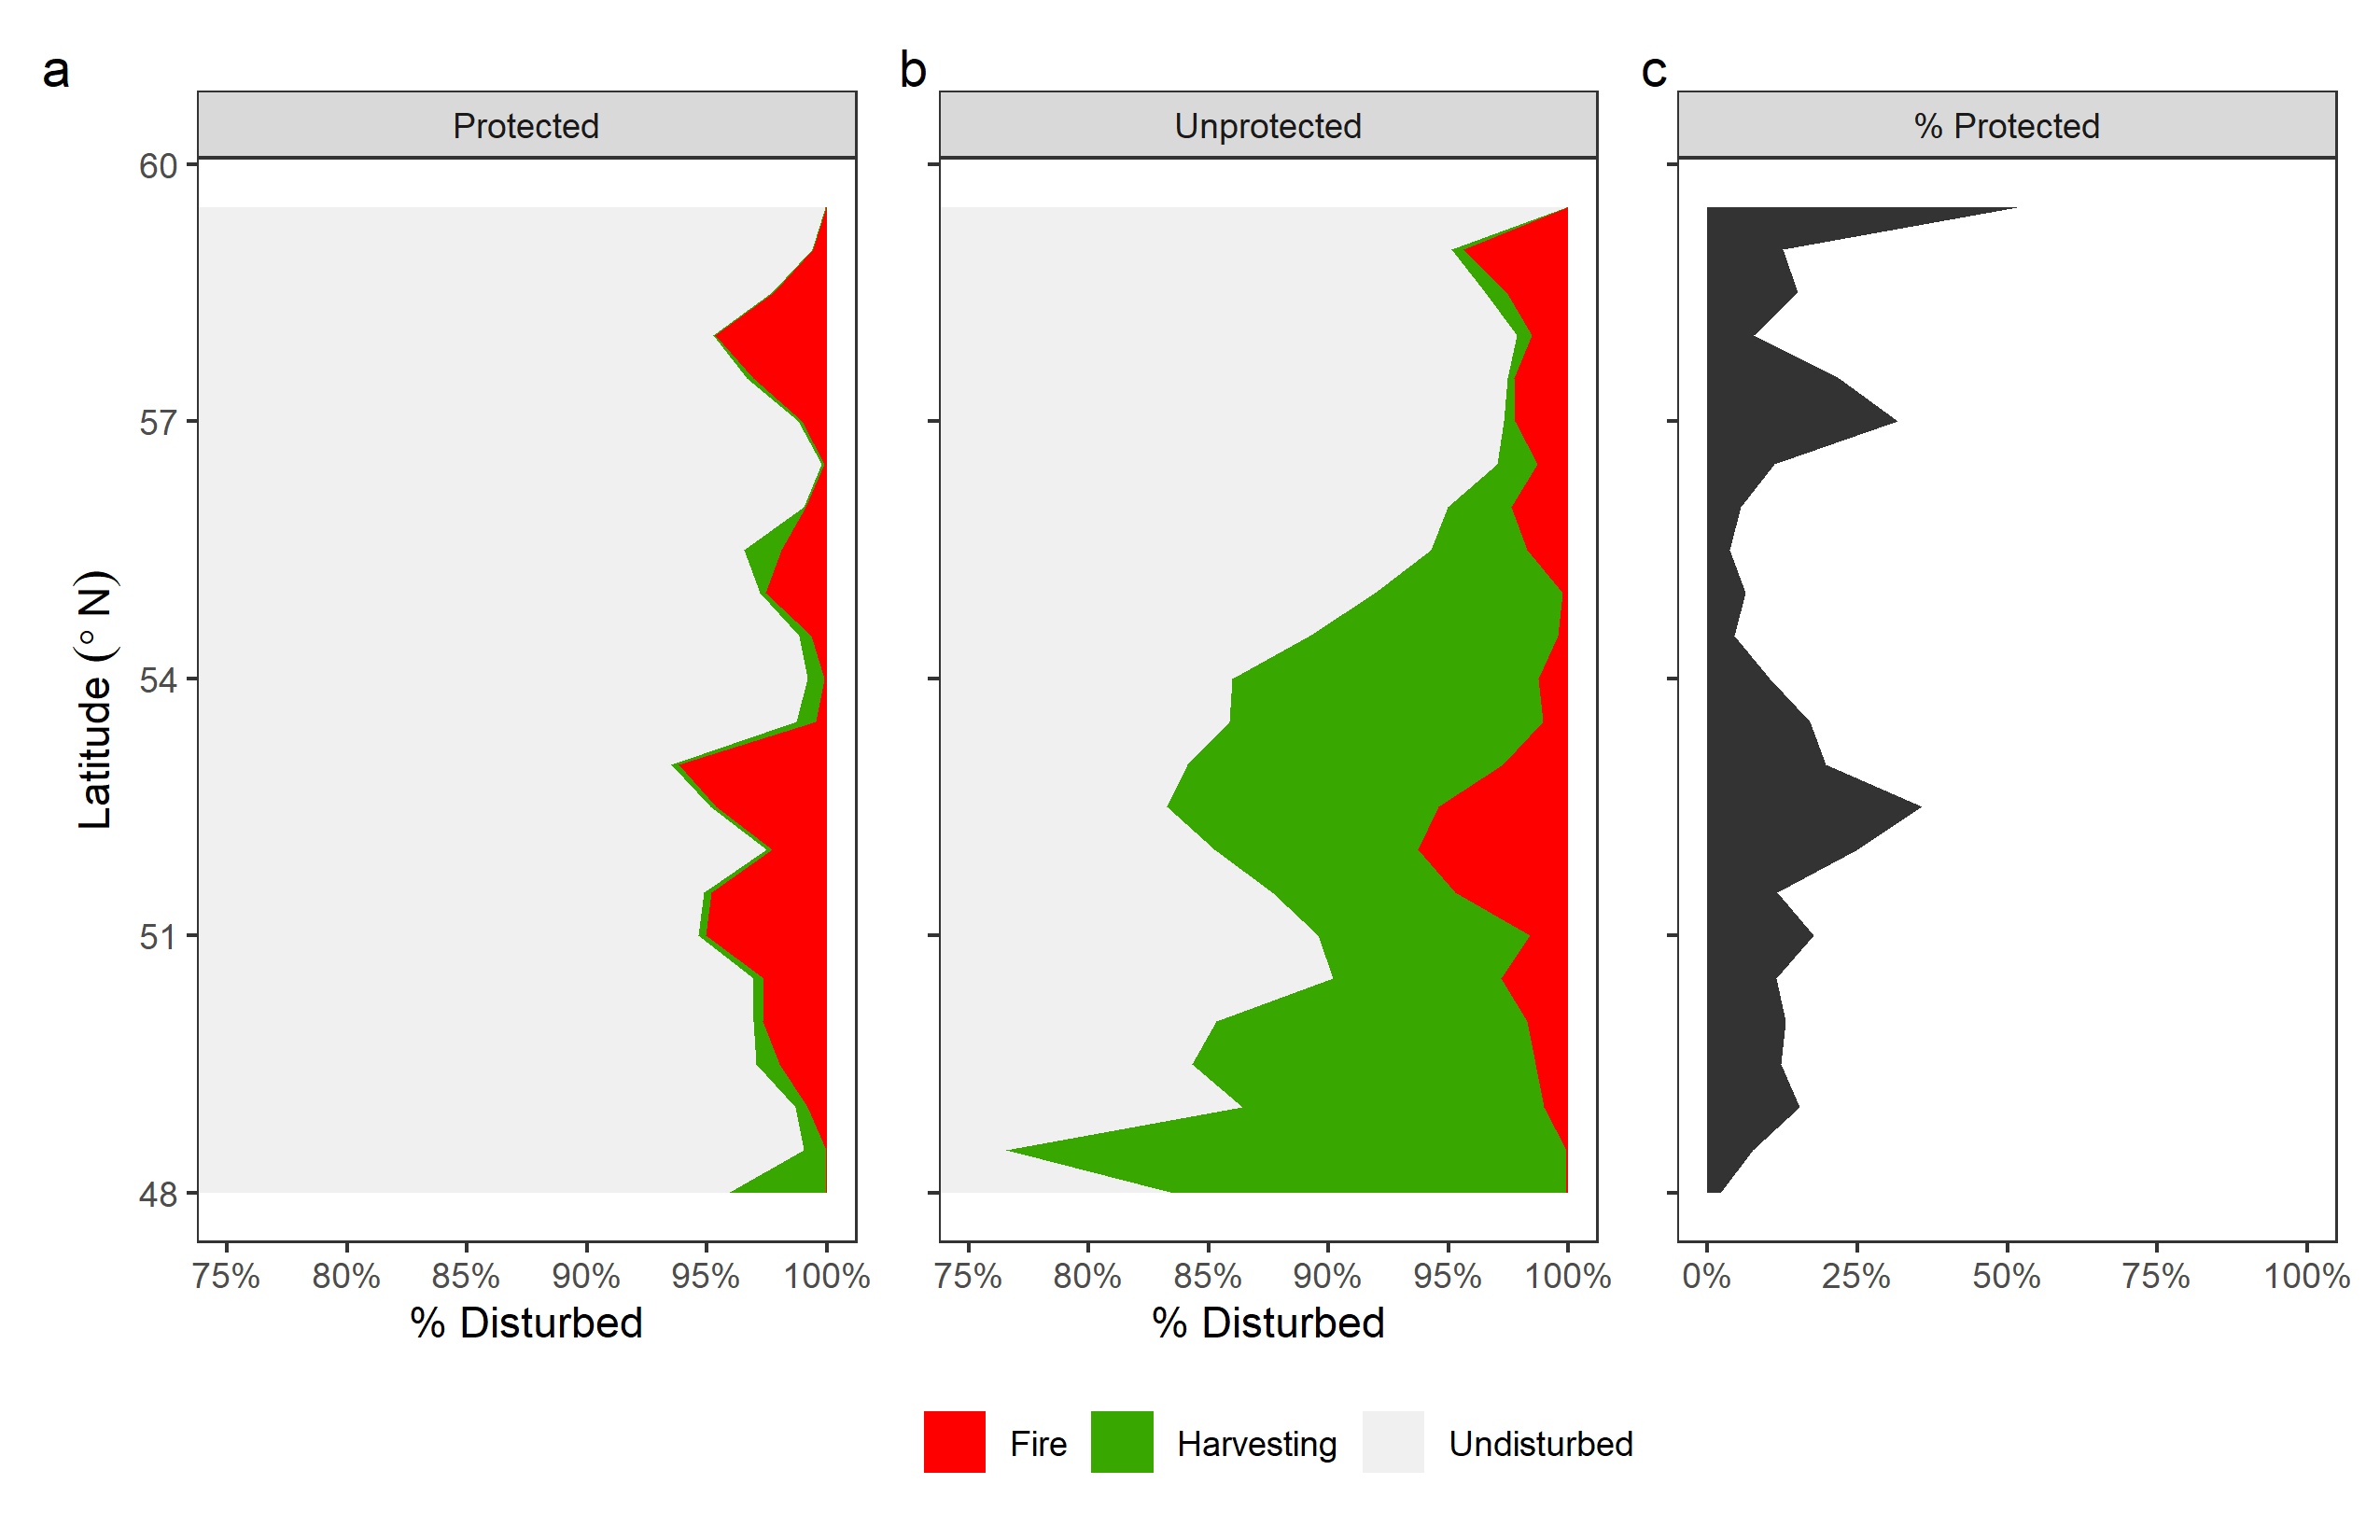
\includegraphics{figures/latitude_disturbance_plot.png}
\caption{Proportion of area disturbed by latitude from 1984 to 2019 in
protected areas (a), and unprotected areas (b). Proportion of
terrestrial area that is protected at each latitude
(c).}\label{fig:lat-dist}
}
\end{figure}

\hypertarget{forest-structural-attributes-1}{%
\subsubsection{Forest Structural
Attributes}\label{forest-structural-attributes-1}}

fig.~\ref{fig:t-test-plot} shows the subzonal proportional significance
(\emph{p \textless{} 0.01}) grouped by ecosystem for the 496 comparisons
of forest structural variables. Higher percentages confirm ecosystems
which had increased number of dissimilar subzones for the specific
indicator, and shows that at least half of all subzones in each
ecosystem are significantly different (the exception being Ponderosa
Pine, which consists of a single subzone that is not significantly
different in canopy structure). Median proportional significance values
for canopy height, canopy cover, and aboveground biomass are universally
significantly different between PA and UA within the same ecosystem.

\begin{figure}
\hypertarget{fig:t-test-plot}{%
\centering
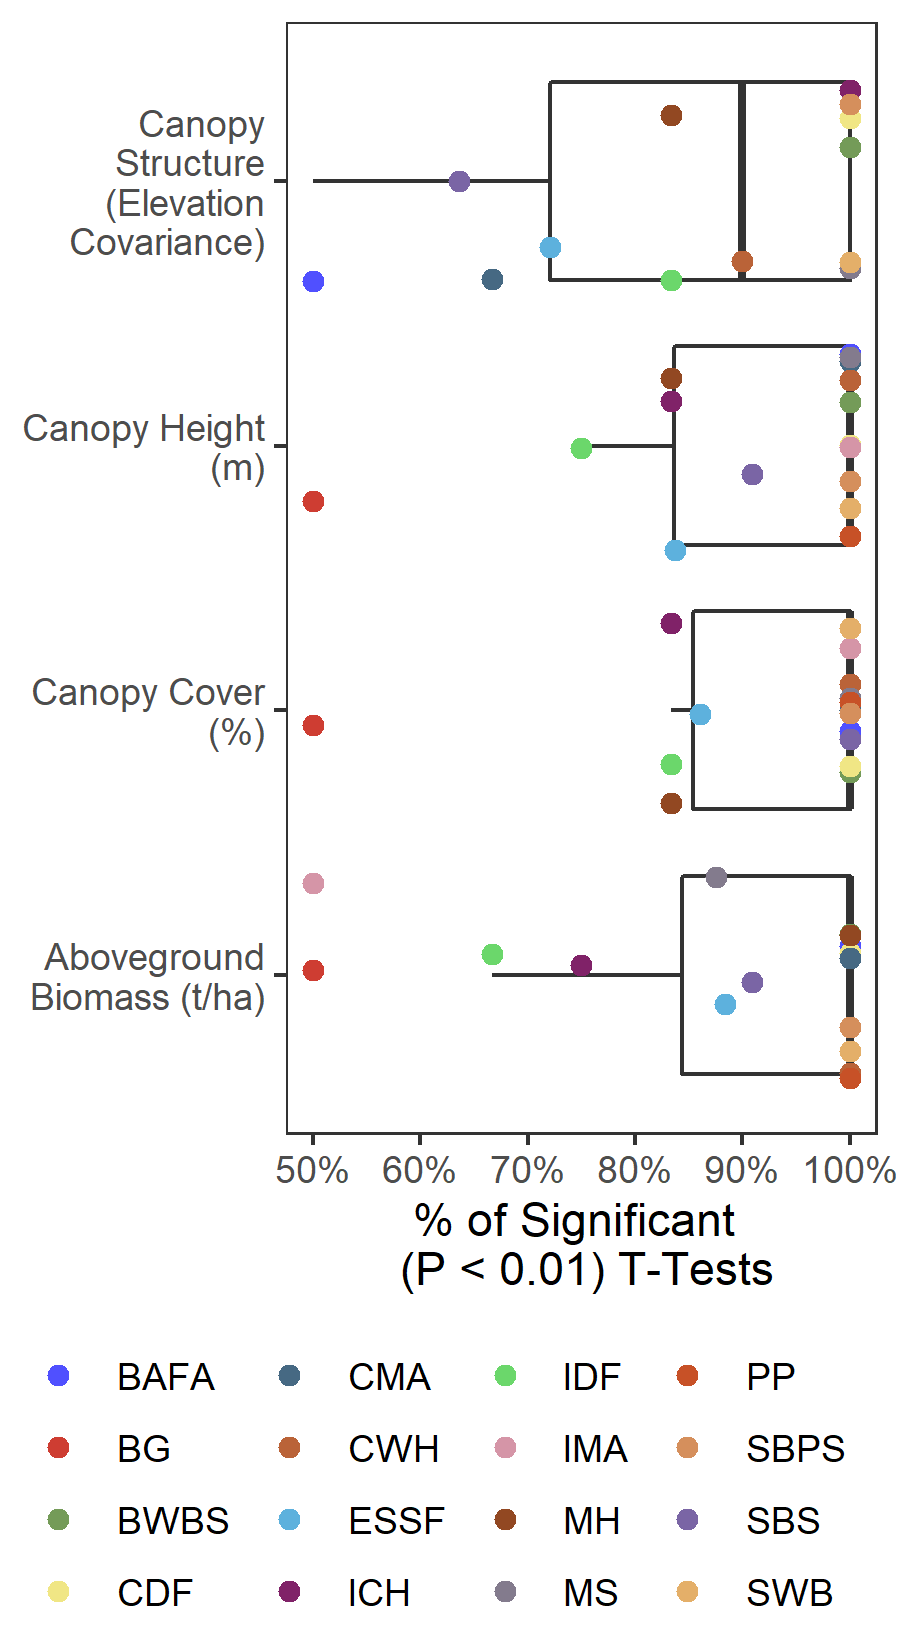
\includegraphics{figures/t_tests_scatter.png}
\caption{Boxplot of proportion of ecosystem subzone which have
significant p-values from a two-tailed t-test with the Bonferroni
correction (n = 496) applied at a significance level of 0.05. Boxplot
vertical lines indicate the first quartile, the median, and the third
quartile. The whisker extends from the first quartile to the smallest
value no further than 1.5 * interquartile range from the first
quartile.}\label{fig:t-test-plot}
}
\end{figure}

Forest structural attributes vary between PA and UA in BC
(fig.~\ref{fig:structure-3d-scatter}). The largest differences between
PA and UA are found in canopy structure in the Coastal Douglas-fir BEC
zone, with the protected area having much higher canopy structure
values. As shown in fig.~\ref{fig:t-test-plot}, forests are commonly
significantly different when comparing PA vs UA across all attributes.
When examining the forests on an BEC zone level, only one BEC zone has a
\textgreater5\% difference in vertical forest structure (co-efficient of
variation in vegetation returns), six BEC zones have \textgreater5\%
difference in canopy cover, and five BEC zones have a \textgreater5\%
difference in canopy height. Ponderosa pine has large differences in
canopy cover and canopy height (\textgreater5\%), but minor differences
in elevation covariance (only 0.25\%; tbl.~\ref{tbl:vector-table}). PA
in the Ponderosa Pine, Interior Mountain Heather Alpine, and Coastal
Douglas-fir have more aboveground biomass than in UA in corresponding
areas (fig.~\ref{fig:structure-3d-scatter}).

Zone

Elevation Covariance

Canopy Cover (\%)

Canopy Height (m)

PA

UA

\% Difference

PA

UA

\% Difference

PA

UA

\% Difference

BAFA

0.39

0.39

0.01\%

46.94\%

48.47\%

3.17\%

14.03

13.11

-7\%

BG

0.38

0.38

-1.41\%

61.8\%

58.71\%

-5.26\%

23.00

21.58

-6.59\%

BWBS

0.37

0.38

2.62\%

67.18\%

64.72\%

-3.8\%

15.83

15.69

-0.9\%

CDF

0.31

0.33

6.35\%

89.38\%

83.69\%

-6.79\%

27.35

26.58

-2.89\%

CMA

0.38

0.39

1.63\%

62.65\%

64.01\%

2.13\%

19.91

20.01

0.48\%

CWH

0.34

0.33

-3.83\%

83.94\%

85.26\%

1.55\%

21.58

22.34

3.4\%

ESSF

0.37

0.37

0.34\%

61.7\%

64.97\%

5.04\%

18.90

18.91

0.07\%

ICH

0.36

0.36

-1.75\%

81.24\%

83.52\%

2.73\%

22.39

22.18

-0.98\%

IDF

0.36

0.36

-0.3\%

67.42\%

67.9\%

0.71\%

21.98

22.49

2.29\%

IMA

0.38

0.36

-3.72\%

68.17\%

62.07\%

-9.83\%

22.53

21.06

-6.98\%

MH

0.36

0.36

0.25\%

76.87\%

77.85\%

1.26\%

19.42

18.31

-6.07\%

MS

0.35

0.35

0.31\%

57.99\%

60.41\%

4.01\%

20.64

20.86

1.04\%

PP

0.36

0.37

0.25\%

57.92\%

48.93\%

-18.36\%

19.88

18.03

-10.24\%

SBPS

0.36

0.35

-1.97\%

32.98\%

34.63\%

4.76\%

18.00

18.70

3.75\%

SBS

0.37

0.37

-0.4\%

62.24\%

67.25\%

7.45\%

18.51

18.67

0.82\%

SWB

0.39

0.39

-1.22\%

56.67\%

57.71\%

1.8\%

13.78

13.67

-0.83\%

: Mean values of forest structural attributes in protected areas (PA),
unprotected areas (UA), as well as the percent difference between the
means. Zones with more than a 5\% difference are bolded.
\{\#tbl:vector-table\}

\begin{figure}
\hypertarget{fig:structure-3d-scatter}{%
\centering
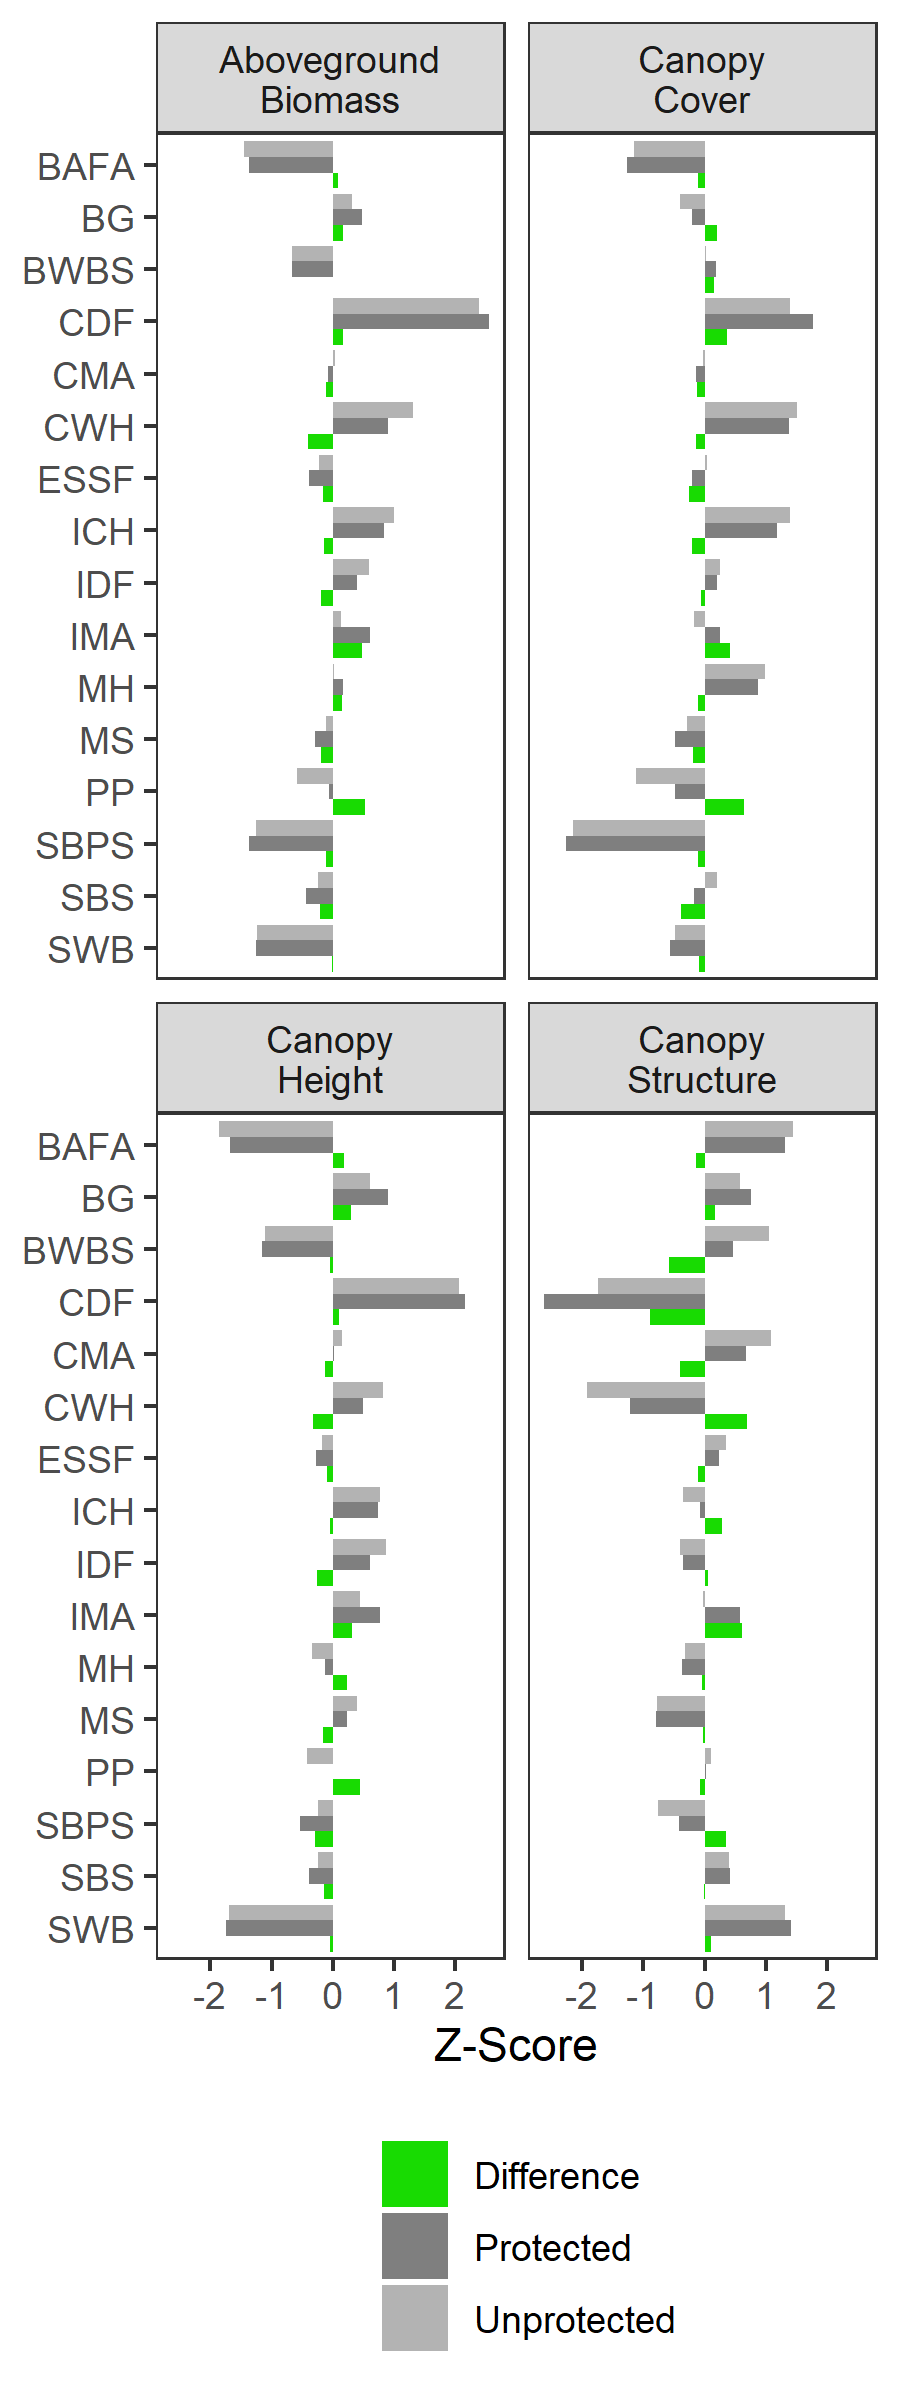
\includegraphics{figures/fstruct_zscores.png}
\caption{Z-Scores of forest structural attributes in PA, UA, and their
differences across BEC zones in BC.}\label{fig:structure-3d-scatter}
}
\end{figure}

\hypertarget{discussion}{%
\section{Discussion}\label{discussion}}

The recent global availability of freely available, open-source,
consistent, and accurate remote sensing data products allow researchers
to examine issues of representation of PA compared to UA, and regional
ecosystems in novel ways (Soverel et al. 2010, Hansen and Phillips 2018,
Bolton et al. 2019). Additionally, the capacity to track forest
structural attributes, a key indicator of forest biodiversity (Guo et
al. 2017), across wide swaths allows for informed decisions on potential
locations of new PA which capture previously underrepresented forest
structure conditions (Noss 1999). By applying this analysis to an entire
PA network across BEC zones (or other ecological classifications), it
becomes possible to determine not only which BEC zones need additional
representation (the proportional metric), but also what types of forest
structures should be represented to ensure adequate biodiversity
protection (Lemieux and Scott 2005).

Internationally, biodiversity preservation targets aim to protect a
proportion of the total terrestrial area (CBD 2010). Frequently, new
protected areas are placed in high-elevation, low-productivity
ecosystems both globally (Joppa and Pfaff 2009, Venter et al. 2014,
2018), and in BC, as confirmed by our analysis of ecosystem
(fig.~\ref{fig:bec-conch}) and land cover (fig.~\ref{fig:vlce-conch})
proportions. Alpine ecosystems are more commonly protected
(fig.~\ref{fig:bec-conch}), as are the land covers commonly present
within them (rock/rubble, snow/ice, exposed/barren land;
fig.~\ref{fig:vlce-conch}). As elevation increases, these ecosystems and
land covers begin to dominate the proportional representation (see
fig.~\ref{fig:bec-elev} and fig.~\ref{fig:lcc-elev}). Differences
between elevation profiles in land cover classes and BEC zones were also
found, with the starkest difference being that wetland classes were
found at lower elevations in PA (fig.~\ref{fig:elev-boxplots})

In high elevation ecosystems, Boreal Altai Fescue Alpine dominates the
PA proportions above 3000m, replacing the Coastal Mountain-Heather
Alpine ecosystem found in UA (fig.~\ref{fig:bec-elev}). These zones were
both protected at rates above the average (fig.~\ref{fig:bec-conch}),
and above the Aichi biodiversity targets. Interior mountain-heather
alpine had large differences in canopy cover and canopy height, while
Boreal Altai Fescue Alpine only showed large differences in height. The
Coastal Mountain-heather Alpine did not any have large forest structural
attribute differences (tbl.~\ref{tbl:vector-table}).

Distribution of disturbances followed a similar pattern to that reported
by Bolton et al. (2019). Thus, the area affected by wildfires is
comparable between PA and UA and at mid latitudes (51-53°N), while
harvesting activity is more prevalent in UA and at low latitudes
(fig.~\ref{fig:lat-dist}).

Our analysis shows that the majority of structural attributes were
significantly different between the protected and unprotected forest
stands across BEC subzones (fig.~\ref{fig:t-test-plot}). In the south,
Coastal Douglas-fir, a zone with a single subzone, had the large
variation between PA and UA in two of four forest structural attributes
examined. The unprotected forests were significantly less tall, had
significantly less canopy cover, and significantly higher elevation
covariance (vertical forest structure;
fig.~\ref{fig:structure-3d-scatter}). In addition, it was the least
protected BEC zone by area, with only 4.9\% of the total terrestrial
area protected. In this specific BEC zone, not only does additional area
need to be protected to meet national goals, different forest structures
need to be included in new protected areas (Paillet et al. 2010).

Utilizing this information on the proportion of BEC zones protected
(fig.~\ref{fig:bec-conch}), as well as their forest structural
attributes (tbl.~\ref{tbl:vector-table}), it is possible to identify
which forest structures need to be added to the PA network in BC. Those
BEC zones with large differences (identified as being \textgreater5\%
change from PA to UA) suggest additional protection is needed to
encapsulate these underrepresented forest structures. For example: the
forests in the Bunchgrass zone have large differences in both canopy
cover and canopy height, with the PA having larger values in both
attributes (tbl.~\ref{tbl:vector-table}). New PA in this BEC zone should
contain forests with shorter and more open forests. A future avenue of
research could be to incorporate forest structural attributes into
spatially optimized PA placement approaches (Christensen et al. 2009).

The advent of free and open-source global datasets can allow for the
monitoring of protected area health across the globe (Nagendra et al.
2013). Analyzing large amounts of free and open-source data using
open-source software approaches offers previously unseen perspectives
into protected area representativeness. There are some challenges
associated with this, namely: optical imagery archives being scarce in
some regions due to imagery acquisition policies (Wulder et al. 2016),
clouds and atmospheric interference, lack of aerial lidar data
available, and varying hierarchies of land cover classifications in
differing regions. New data and satellite missions are being introduced
that can meet these challenges at a spatial resolution of 30 m or less
such as Landsat-9 and Sentinel-2, as well as spaceborne lidar such as
GEDI (Dubayah et al. 2020) and ICESat-2 (Neuenschwander et al. 2020),
which can provide global coverage of various forest structural
attributes (Potapov et al. 2021) through similar imputation methods to
Matasci et al. (2018a), global land cover maps (Potapov et al. 2020,
Zanaga et al. 2021), and forest disturbance maps (Hansen et al. 2013).
These novel datasets provide clear opportunities for regional to global
analyses of PA vs UA to be conducted concerning forest structure.

Future research monitoring protected area health using satellite remote
sensing could focus on implementing essential biodiversity variables
(Pereira et al. 2013) into their monitoring scheme. Advancing research
towards these variables would not only benefit PA monitoring projects,
but also biodiversity monitoring projects across the globe. Beyond this,
examining the recovery of forest structural attribute following
disturbances in both PA and UA could assess the effectiveness of PA for
promoting regeneration.

\hypertarget{conclusion}{%
\section{Conclusion}\label{conclusion}}

In conclusion, we identified biases in the BC PA network for PA to be
placed in high-elevation BEC zones, commonly dominated by
low-productivity land covers. We examined the disturbance regimes of PA
vs UA by latitude, finding that wildfires are similar, while harvesting
differs across the province. We then compared the forest structural
attributes across all BEC subzones, finding that the majority of
subzones have significantly different forest structures. Beyond this, we
identified BEC zones with large variation in mean forest structural
attributes. When new PA locations are decided upon in BC, they should
take forest structure into consideration, as wall-to-wall coverage of
forest structural attributes becomes available. Novel datasets can allow
this methodology to be applied across large regions, in order to
identify PA biases and underrepresented forest structures.

\newpage

\hypertarget{acknowledgments}{%
\section{Acknowledgments}\label{acknowledgments}}

This research was funded through the Living Lab for Climate Change and
Conservation program of the British Columbia Parks (grant ID:
TP21JHQ011) and in part by NSERC support of Coops (RGPIN-2018-03851).
Remote sensing data products utilized in this research are free and open
and available for download at: \url{https://ca.nfis.org/maps_eng.html}.
We thank Dr Michael Wulder and Dr Joanne White for development and early
access to these National Terrestrial Ecosystem Mapping System (NTEMS)
products. We also thank an anonymous reviewer for their comments which
helped improve the manuscript.

\hypertarget{literature-cited}{%
\section*{Literature Cited}\label{literature-cited}}
\addcontentsline{toc}{section}{Literature Cited}

\hypertarget{refs}{}
\begin{CSLReferences}{1}{0}
\leavevmode\hypertarget{ref-alsdorf2007}{}%
Alsdorf, D. E., E. Rodriguez, and D. P. Lettenmaier. 2007. Measuring
surface water from space. Reviews of Geophysics 45:RG2002.

\leavevmode\hypertarget{ref-bcministryofforestsBritishColumbiaForests2003}{}%
BC Ministry of Forests. 2003. British Columbia's forests and their
management.

\leavevmode\hypertarget{ref-bcparks2012}{}%
BC Parks. 2012. Ecological Integrity in British Columbia's Parks and
Protected Areas.

\leavevmode\hypertarget{ref-boltonUncoveringRegionalVariability2019}{}%
Bolton, D. K., N. C. Coops, T. Hermosilla, M. A. Wulder, J. C. White,
and C. J. Ferster. 2019. Uncovering regional variability in disturbance
trends between parks and greater park ecosystems across Canada (1985).
Scientific Reports 9:1323.

\leavevmode\hypertarget{ref-bonferroni1936}{}%
Bonferroni, C. E. 1936. Teoria statistica delle classi e calcolo delle
probabilità. Pages 3--62.

\leavevmode\hypertarget{ref-brooks2004}{}%
Brooks, T. M., M. I. Bakarr, T. Boucher, G. A. B. Da Fonseca, C.
Hilton-Taylor, J. M. Hoekstra, T. Moritz, S. Olivieri, J. Parrish, R. L.
Pressey, A. S. L. Rodrigues, W. Sechrest, A. Stattersfield, W. Strahm,
and S. N. Stuart. 2004. Coverage Provided by the Global Protected-Area
System: Is It Enough? BioScience 54:1081.

\leavevmode\hypertarget{ref-buchanan2018}{}%
Buchanan, G. M., A. E. Beresford, M. Hebblewhite, F. J. Escobedo, H. M.
D. Klerk, P. F. Donald, P. Escribano, L. P. Koh, J. Martínez-López, N.
Pettorelli, A. K. Skidmore, Z. Szantoi, K. Tabor, M. Wegmann, and S.
Wich. 2018. Free satellite data key to conservation. Science
361:139--140.

\leavevmode\hypertarget{ref-burkhardMappingEcosystemService2012}{}%
Burkhard, B., F. Kroll, S. Nedkov, and F. Müller. 2012. Mapping
ecosystem service supply, demand and budgets. Ecological Indicators
21:17--29.

\leavevmode\hypertarget{ref-butchart2015}{}%
Butchart, S. H. M., M. Clarke, R. J. Smith, R. E. Sykes, J. P. W.
Scharlemann, M. Harfoot, G. M. Buchanan, A. Angulo, A. Balmford, B.
Bertzky, T. M. Brooks, K. E. Carpenter, M. T. Comeros-Raynal, J.
Cornell, G. F. Ficetola, L. D. C. Fishpool, R. A. Fuller, J. Geldmann,
H. Harwell, C. Hilton-Taylor, M. Hoffmann, A. Joolia, L. Joppa, N.
Kingston, I. May, A. Milam, B. Polidoro, G. Ralph, N. Richman, C.
Rondinini, D. B. Segan, B. Skolnik, M. D. Spalding, S. N. Stuart, A.
Symes, J. Taylor, P. Visconti, J. E. M. Watson, L. Wood, and N. D.
Burgess. 2015. Shortfalls and Solutions for Meeting National and Global
Conservation Area Targets. Conservation Letters 8:329--337.

\leavevmode\hypertarget{ref-cbd2004}{}%
CBD. 2004. CoP 7 decision VII/30. Strategic plan: future evaluation of
progress. Goal 1 promote the conservation of the biological diversity of
ecosystems, habitats and biomes; Target 1.1.

\leavevmode\hypertarget{ref-cbd2010}{}%
CBD. 2010. The strategic plan for biodiversity 2011-2020 and the Aichi
biodiversity targests.

\leavevmode\hypertarget{ref-chapeMeasuringExtentEffectiveness2005}{}%
Chape, S., J. Harrison, M. Spalding, and I. Lysenko. 2005. Measuring the
extent and effectiveness of protected areas as an indicator for meeting
global biodiversity targets. Philosophical Transactions of the Royal
Society B: Biological Sciences 360:443--455.

\leavevmode\hypertarget{ref-christensen2009}{}%
Christensen, V., Z. Ferdaña, and J. Steenbeek. 2009. Spatial
optimization of protected area placement incorporating ecological,
social and economical criteria. Ecological Modelling 220:2583--2593.

\leavevmode\hypertarget{ref-coadMeasuringImpactProtected2015}{}%
Coad, L., F. Leverington, K. Knights, J. Geldmann, A. Eassom, V. Kapos,
N. Kingston, M. de Lima, C. Zamora, I. Cuardros, C. Nolte, N. D.
Burgess, and M. Hockings. 2015. Measuring impact of protected area
management interventions: Current and future use of the global database
of protected area management effectiveness. Philosophical Transactions
of the Royal Society B: Biological Sciences 370:20140281.

\leavevmode\hypertarget{ref-cohen2004}{}%
Cohen, W. B., and S. N. Goward. 2004. Landsat's role in ecological
applications of remote sensing. Bioscience 54:535--545.

\leavevmode\hypertarget{ref-defries2005}{}%
Defries, R., A. Hansen, A. Newton, and M. Hansen. 2005. Increasing
isolation of protected areas in tropical forests over the past twenty
years. Ecological Applications 15:19--26.

\leavevmode\hypertarget{ref-dinersteinEcoregionBasedApproachProtecting2017}{}%
Dinerstein, E., D. Olson, A. Joshi, C. Vynne, N. D. Burgess, E.
Wikramanayake, N. Hahn, S. Palminteri, P. Hedao, R. Noss, M. Hansen, H.
Locke, E. C. Ellis, B. Jones, C. V. Barber, R. Hayes, C. Kormos, V.
Martin, E. Crist, W. Sechrest, L. Price, J. E. M. Baillie, D. Weeden, K.
Suckling, C. Davis, N. Sizer, R. Moore, D. Thau, T. Birch, P. Potapov,
S. Turubanova, A. Tyukavina, N. de Souza, L. Pintea, J. C. Brito, O. A.
Llewellyn, A. G. Miller, A. Patzelt, S. A. Ghazanfar, J. Timberlake, H.
Klöser, Y. Shennan-Farpón, R. Kindt, J.-P. B. Lillesø, P. van Breugel,
L. Graudal, M. Voge, K. F. Al-Shammari, and M. Saleem. 2017. An
Ecoregion-Based Approach to Protecting Half the Terrestrial Realm.
BioScience 67:534--545.

\leavevmode\hypertarget{ref-dinerstein2019}{}%
Dinerstein, E., C. Vynne, E. Sala, A. R. Joshi, S. Fernando, T. E.
Lovejoy, J. Mayorga, D. Olson, G. P. Asner, J. E. M. Baillie, N. D.
Burgess, K. Burkart, R. F. Noss, Y. P. Zhang, A. Baccini, T. Birch, N.
Hahn, L. N. Joppa, and E. Wikramanayake. 2019. A Global Deal For Nature:
Guiding principles, milestones, and targets. Science Advances
5:eaaw2869.

\leavevmode\hypertarget{ref-dubayahGlobalEcosystemDynamics2020}{}%
Dubayah, R., J. B. Blair, S. Goetz, L. Fatoyinbo, M. Hansen, S. Healey,
M. Hofton, G. Hurtt, J. Kellner, S. Luthcke, J. Armston, H. Tang, L.
Duncanson, S. Hancock, P. Jantz, S. Marselis, P. L. Patterson, W. Qi,
and C. Silva. 2020. The Global Ecosystem Dynamics Investigation:
High-resolution laser ranging of the Earth's forests and topography.
Science of Remote Sensing 1:100002.

\leavevmode\hypertarget{ref-eccc2021}{}%
ECCC. 2021, May 3. Canada Target 1 Challenge.

\leavevmode\hypertarget{ref-eklundWhatConstitutesUseful2019}{}%
Eklund, J., L. Coad, J. Geldmann, and M. Cabeza. 2019. What constitutes
a useful measure of protected area effectiveness? A case study of
management inputs and protected area impacts in Madagascar. Conservation
Science and Practice 1:e107.

\leavevmode\hypertarget{ref-environmentalreportingbc2016}{}%
Environmental Reporting BC. 2016. Protected Lands and Waters in British
Columbia.
http://www.env.gov.bc.ca/soe/indicators/land/protected-lands-and-waters.html.

\leavevmode\hypertarget{ref-feeley2005}{}%
Feeley, K. J., T. W. Gillespie, and J. W. Terborgh. 2005. The Utility of
Spectral Indices from Landsat ETM+ for Measuring the Structure and
Composition of Tropical Dry Forests. Biotropica 37:508--519.

\leavevmode\hypertarget{ref-ferraroCounterfactualThinkingImpact2009}{}%
Ferraro, P. J. 2009. Counterfactual thinking and impact evaluation in
environmental policy. New Directions for Evaluation 2009:75--84.

\leavevmode\hypertarget{ref-fraserMonitoringLandCover2009}{}%
Fraser, R. H., I. Olthof, and D. Pouliot. 2009. Monitoring land cover
change and ecological integrity in Canada's national parks. Remote
Sensing of Environment 113:1397--1409.

\leavevmode\hypertarget{ref-gao2014}{}%
Gao, T., M. Hedblom, T. Emilsson, and A. B. Nielsen. 2014. The role of
forest stand structure as biodiversity indicator. Forest Ecology and
Management 330:82--93.

\leavevmode\hypertarget{ref-gastonEcologicalEffectivenessProtected2006}{}%
Gaston, K. J., K. Charman, S. F. Jackson, P. R. Armsworth, A. Bonn, R.
A. Briers, C. S. Q. Callaghan, R. Catchpole, J. Hopkins, W. E. Kunin, J.
Latham, P. Opdam, R. Stoneman, D. A. Stroud, and R. Tratt. 2006. The
ecological effectiveness of protected areas: The United Kingdom.
Biological Conservation 132:76--87.

\leavevmode\hypertarget{ref-gastonEcologicalPerformanceProtected2008}{}%
Gaston, K. J., S. F. Jackson, L. Cantú-Salazar, and G. Cruz-Piñón. 2008.
The Ecological Performance of Protected Areas. Annual Review of Ecology,
Evolution, and Systematics 39:93--113.

\leavevmode\hypertarget{ref-geldmannGloballevelAssessmentEffectiveness2019}{}%
Geldmann, J., A. Manica, N. D. Burgess, L. Coad, and A. Balmford. 2019.
A global-level assessment of the effectiveness of protected areas at
resisting anthropogenic pressures. Proceedings of the National Academy
of Sciences 116:23209--23215.

\leavevmode\hypertarget{ref-gillespie2005}{}%
Gillespie, T. W. 2005. Predicting Woody-Plant Species Richness in
Tropical Dry Forests: A Case Study from South Florida, Usa. Ecological
Applications 15:27--37.

\leavevmode\hypertarget{ref-goetz2007}{}%
Goetz, S., D. Steinberg, R. Dubayah, and B. Blair. 2007. Laser remote
sensing of canopy habitat heterogeneity as a predictor of bird species
richness in an eastern temperate forest, USA. Remote Sensing of
Environment 108:254--263.

\leavevmode\hypertarget{ref-governmentofcanada2019}{}%
Government of Canada,. 2019, September 4. Canada National Park Act.

\leavevmode\hypertarget{ref-guo2017}{}%
Guo, X., N. C. Coops, P. Tompalski, S. E. Nielsen, C. W. Bater, and J.
John Stadt. 2017. Regional mapping of vegetation structure for
biodiversity monitoring using airborne lidar data. Ecological
Informatics 38:50--61.

\leavevmode\hypertarget{ref-hamann2005}{}%
Hamann, A., P. Smets, A. D. Yanchuk, and S. N. Aitken. 2005. An
ecogeographic framework for in situ conservation of forest trees in
British Columbia. Canadian Journal of Forest Research 35:2553--2561.

\leavevmode\hypertarget{ref-hansenMonitoringForestEcosystem2021}{}%
Hansen, A. J., B. P. Noble, J. Veneros, A. East, S. J. Goetz, C.
Supples, J. E. M. Watson, P. A. Jantz, R. Pillay, W. Jetz, S. Ferrier,
H. S. Grantham, T. D. Evans, J. Ervin, O. Venter, and A. L. S. Virnig.
2021. Toward monitoring forest ecosystem integrity within the post-2020
Global Biodiversity Framework. Conservation Letters 14:e12822.

\leavevmode\hypertarget{ref-hansenTrendsVitalSigns2018}{}%
Hansen, A. J., and L. Phillips. 2018. Trends in vital signs for Greater
Yellowstone: Application of a Wildland Health Index. Ecosphere 9:e02380.

\leavevmode\hypertarget{ref-hansenHighResolutionGlobalMaps2013}{}%
Hansen, M. C., P. V. Potapov, R. Moore, M. Hancher, S. A. Turubanova, A.
Tyukavina, D. Thau, S. V. Stehman, S. J. Goetz, T. R. Loveland, A.
Kommareddy, A. Egorov, L. Chini, C. O. Justice, and J. R. G. Townshend.
2013. High-Resolution Global Maps of 21st-Century Forest Cover Change.
Science 342:850--853.

\leavevmode\hypertarget{ref-hazen2004}{}%
Hazen, H. D., and P. J. Anthamatten. 2004. Representation of ecological
regions by protected areas at the global scale. Physical Geography
25:499--512.

\leavevmode\hypertarget{ref-hermosillaIntegratedLandsatTime2015}{}%
Hermosilla, T., M. A. Wulder, J. C. White, N. C. Coops, and G. W.
Hobart. 2015a. An integrated Landsat time series protocol for change
detection and generation of annual gap-free surface reflectance
composites. Remote Sensing of Environment 158:220--234.

\leavevmode\hypertarget{ref-hermosilla2015}{}%
Hermosilla, T., M. A. Wulder, J. C. White, N. C. Coops, and G. W.
Hobart. 2015b. Regional detection, characterization, and attribution of
annual forest change from 1984 to 2012 using landsat-derived time-series
metrics. Remote Sensing of Environment 170:121132.

\leavevmode\hypertarget{ref-hermosillaDisturbanceInformedAnnualLand2018}{}%
Hermosilla, T., M. A. Wulder, J. C. White, N. C. Coops, and G. W.
Hobart. 2018. Disturbance-Informed Annual Land Cover Classification Maps
of Canada's Forested Ecosystems for a 29-Year Landsat Time Series.
Canadian Journal of Remote Sensing 44:67--87.

\leavevmode\hypertarget{ref-hermosillaMassDataProcessing2016}{}%
Hermosilla, T., M. A. Wulder, J. C. White, N. C. Coops, G. W. Hobart,
and L. B. Campbell. 2016. Mass data processing of time series Landsat
imagery: Pixels to data products for forest monitoring. International
Journal of Digital Earth 9:1035--1054.

\leavevmode\hypertarget{ref-joppa2009}{}%
Joppa, L. N., and A. Pfaff. 2009. High and Far: Biases in the Location
of Protected Areas. PLOS ONE 4:e8273.

\leavevmode\hypertarget{ref-kerr2003}{}%
Kerr, J. T., and M. Ostrovsky. 2003. From space to species: ecological
applications for remote sensing. Trends in Ecology \& Evolution
18:299--305.

\leavevmode\hypertarget{ref-lemieux2005}{}%
Lemieux, C. J., and D. J. Scott. 2005. Climate change, biodiversity
conservation and protected area planning in Canada. The Canadian
Geographer / Le Géographe canadien 49:384--397.

\leavevmode\hypertarget{ref-lim2003}{}%
Lim, K., P. Treitz, M. Wulder, B. St-Onge, and M. Flood. 2003. LiDAR
remote sensing of forest structure. Progress in Physical Geography:
Earth and Environment 27:88--106.

\leavevmode\hypertarget{ref-lucas2011}{}%
Lucas, R., K. Medcalf, A. Brown, P. Bunting, J. Breyer, D. Clewley, S.
Keyworth, and P. Blackmore. 2011. Updating the Phase 1 habitat map of
Wales, UK, using satellite sensor data. ISPRS Journal of Photogrammetry
and Remote Sensing 66:81--102.

\leavevmode\hypertarget{ref-matasciThreeDecadesForest2018}{}%
Matasci, G., T. Hermosilla, M. A. Wulder, J. C. White, N. C. Coops, G.
W. Hobart, D. K. Bolton, P. Tompalski, and C. W. Bater. 2018a. Three
decades of forest structural dynamics over Canada's forested ecosystems
using Landsat time-series and lidar plots. Remote Sensing of Environment
216:697--714.

\leavevmode\hypertarget{ref-matasciLargeareaMappingCanadian2018}{}%
Matasci, G., T. Hermosilla, M. A. Wulder, J. C. White, N. C. Coops, G.
W. Hobart, and H. S. J. Zald. 2018b. Large-area mapping of Canadian
boreal forest cover, height, biomass and other structural attributes
using Landsat composites and lidar plots. Remote Sensing of Environment
209:90--106.

\leavevmode\hypertarget{ref-maxwell2020}{}%
Maxwell, S. L., V. Cazalis, N. Dudley, M. Hoffmann, A. S. L. Rodrigues,
S. Stolton, P. Visconti, S. Woodley, N. Kingston, E. Lewis, M. Maron, B.
B. N. Strassburg, A. Wenger, H. D. Jonas, O. Venter, and J. E. M.
Watson. 2020. Area-based conservation in the twenty-first century.
Nature 586:217--227.

\leavevmode\hypertarget{ref-mcdermid2005}{}%
McDermid, G. J., S. E. Franklin, and E. F. LeDrew. 2005. Remote sensing
for large-area habitat mapping. Progress in Physical Geography: Earth
and Environment 29:449--474.

\leavevmode\hypertarget{ref-meidingerEcosystemsBritishColumbia1991}{}%
Meidinger, D. V., and J. Pojar, editors. 1991. Ecosystems of British
Columbia. Research Branch, Ministry of Forests, Victoria, B.C.

\leavevmode\hypertarget{ref-myneni2001}{}%
Myneni, R. B., J. Dong, C. J. Tucker, R. K. Kaufmann, P. E. Kauppi, J.
Liski, L. Zhou, V. Alexeyev, and M. K. Hughes. 2001. A large carbon sink
in the woody biomass of northern forests. Proceedings of the National
Academy of Sciences of the United States of America 98:14784--14789.

\leavevmode\hypertarget{ref-nagendra2001}{}%
Nagendra, H. 2001. Using remote sensing to assess biodiversity.
International Journal of Remote Sensing 22:2377--2400.

\leavevmode\hypertarget{ref-nagendraParksWorkImpact2008}{}%
Nagendra, H. 2008. Do parks work? Impact of protected areas on land
cover clearing. Ambio 37:330--337.

\leavevmode\hypertarget{ref-nagendraRemoteSensingConservation2013}{}%
Nagendra, H., R. Lucas, J. P. Honrado, R. H. G. Jongman, C. Tarantino,
M. Adamo, and P. Mairota. 2013. Remote sensing for conservation
monitoring: Assessing protected areas, habitat extent, habitat
condition, species diversity, and threats. Ecological Indicators
33:45--59.

\leavevmode\hypertarget{ref-nagendra2010}{}%
Nagendra, H., D. Rocchini, R. Ghate, B. Sharma, and S. Pareeth. 2010.
Assessing Plant Diversity in a Dry Tropical Forest: Comparing the
Utility of Landsat and Ikonos Satellite Images. Remote Sensing
2:478--496.

\leavevmode\hypertarget{ref-neuenschwander2020}{}%
Neuenschwander, A., E. Guenther, J. C. White, L. Duncanson, and P.
Montesano. 2020. Validation of ICESat-2 terrain and canopy heights in
boreal forests. Remote Sensing of Environment 251:112110.

\leavevmode\hypertarget{ref-noss1999}{}%
Noss, R. F. 1999. Assessing and monitoring forest biodiversity: A
suggested framework and indicators. Forest Ecology and Management
115:135--146.

\leavevmode\hypertarget{ref-olthofUsingSatelliteRemote2006}{}%
Olthof, I., D. Pouliot, R. Fraser, A. Clouston, S. Wang, W. Chen, J.
Orazietti, J. Poitevin, D. Mclennan, J. Kerr, and M. Sawada. 2006. Using
Satellite Remote Sensing to Assess and Monitor Ecosystem Integrity and
Climate Change in Canadas National Parks. 2006 IEEE International
Symposium on Geoscience and Remote Sensing. IEEE.

\leavevmode\hypertarget{ref-paillet2010}{}%
Paillet, Y., L. Berges, J. Hjalten, P. Odor, C. Avon, M.
Bernhardt-Roemermann, R.-J. Bijlsma, L. De Bruyn, M. Fuhr, U. Grandin,
R. Kanka, L. Lundin, S. Luque, T. Magura, S. Matesanz, I. Meszaros, M.-.
Teresa Sebastia, W. Schmidt, T. Standovar, B. Tothmeresz, A. Uotila, F.
Valladares, K. Vellak, and R. Virtanen. 2010. Biodiversity differences
between managed and unmanaged forests: Meta-analysis of species richness
in europe. Conservation Biology 24:101--112.

\leavevmode\hypertarget{ref-parkscanadaEcologicalIntegrity2019}{}%
Parks Canada. 2019. Ecological Integrity.
https://www.pc.gc.ca/en/nature/science/conservation/ie-ei.

\leavevmode\hypertarget{ref-parmenterLandUseLand2003}{}%
Parmenter, A. W., A. Hansen, R. E. Kennedy, W. Cohen, U. Langner, R.
Lawrence, B. Maxwell, A. Gallant, and R. Aspinall. 2003. Land use and
land cover change in the Greater Yellowstone Ecosystem: 1975. Ecological
Applications 13:687--703.

\leavevmode\hypertarget{ref-parrishAreWeConserving2003}{}%
Parrish, J. D., D. P. Braun, and R. S. Unnasch. 2003. Are We Conserving
What We Say We Are? Measuring Ecological Integrity within Protected
Areas. BioScience 53:851.

\leavevmode\hypertarget{ref-pereira2013}{}%
Pereira, H. M., S. Ferrier, M. Walters, G. N. Geller, R. H. G. Jongman,
R. J. Scholes, M. W. Bruford, N. Brummitt, S. H. M. Butchart, A. C.
Cardoso, N. C. Coops, E. Dulloo, D. P. Faith, J. Freyhof, R. D. Gregory,
C. Heip, R. Hoft, G. Hurtt, W. Jetz, D. S. Karp, M. A. McGeoch, D.
Obura, Y. Onoda, N. Pettorelli, B. Reyers, R. Sayre, J. P. W.
Scharlemann, S. N. Stuart, E. Turak, M. Walpole, and M. Wegmann. 2013.
Essential Biodiversity Variables. Science 339:277--278.

\leavevmode\hypertarget{ref-pojarBiogeoclimaticEcosystemClassification1987}{}%
Pojar, J., K. Klinka, and D. V. Meidinger. 1987. Biogeoclimatic
ecosystem classification in British Columbia. Forest Ecology and
Management 22:119--154.

\leavevmode\hypertarget{ref-potapovLandsatAnalysisReady2020}{}%
Potapov, P., M. C. Hansen, I. Kommareddy, A. Kommareddy, S. Turubanova,
A. Pickens, B. Adusei, A. Tyukavina, and Q. Ying. 2020. Landsat Analysis
Ready Data for Global Land Cover and Land Cover Change Mapping. Remote
Sensing 12:426.

\leavevmode\hypertarget{ref-potapovMappingGlobalForest2021}{}%
Potapov, P., X. Li, A. Hernandez-Serna, A. Tyukavina, M. C. Hansen, A.
Kommareddy, A. Pickens, S. Turubanova, H. Tang, C. E. Silva, J. Armston,
R. Dubayah, J. B. Blair, and M. Hofton. 2021. Mapping global forest
canopy height through integration of GEDI and Landsat data. Remote
Sensing of Environment 253:112165.

\leavevmode\hypertarget{ref-puxf4uxe7as2011}{}%
Pôças, I., M. Cunha, and L. S. Pereira. 2011. Remote sensing based
indicators of changes in a mountain rural landscape of Northeast
Portugal. Applied Geography 31:871--880.

\leavevmode\hypertarget{ref-R-base}{}%
R Core Team. 2021. R: A language and environment for statistical
computing. R Foundation for Statistical Computing, Vienna, Austria.

\leavevmode\hypertarget{ref-ribasGlobalComparativeAnalysis2020}{}%
Ribas, L. G. dos S., R. L. Pressey, R. Loyola, and L. M. Bini. 2020. A
global comparative analysis of impact evaluation methods in estimating
the effectiveness of protected areas. Biological Conservation
246:108595.

\leavevmode\hypertarget{ref-rocchini2010}{}%
Rocchini, D., N. Balkenhol, G. A. Carter, G. M. Foody, T. W. Gillespie,
K. S. He, S. Kark, N. Levin, K. Lucas, M. Luoto, H. Nagendra, J.
Oldeland, C. Ricotta, J. Southworth, and M. Neteler. 2010. Remotely
sensed spectral heterogeneity as a proxy of species diversity: Recent
advances and open challenges. Ecological Informatics 5:318--329.

\leavevmode\hypertarget{ref-running2004}{}%
Running, S. W., R. R. Nemani, F. A. Heinsch, M. S. Zhao, M. Reeves, and
H. Hashimoto. 2004. A continuous satellite-derived measure of global
terrestrial primary production. Bioscience 54:547--560.

\leavevmode\hypertarget{ref-skidmore2021}{}%
Skidmore, A. K., N. C. Coops, E. Neinavaz, A. Ali, M. E. Schaepman, M.
Paganini, W. D. Kissling, P. Vihervaara, R. Darvishzadeh, H. Feilhauer,
M. Fernandez, N. Fernández, N. Gorelick, I. Geijzendorffer, U. Heiden,
M. Heurich, D. Hobern, S. Holzwarth, F. E. Muller-Karger, R. Van De
Kerchove, A. Lausch, P. J. Leitão, M. C. Lock, C. A. Mücher, B.
O'Connor, D. Rocchini, W. Turner, J. K. Vis, T. Wang, M. Wegmann, and V.
Wingate. 2021. Priority list of biodiversity metrics to observe from
space. Nature Ecology \& Evolution.

\leavevmode\hypertarget{ref-soverelCharacterizingForestFragmentation2010}{}%
Soverel, N. O., N. C. Coops, J. C. White, and M. A. Wulder. 2010.
Characterizing the forest fragmentation of Canada's national parks.
Environmental Monitoring and Assessment 164:481--499.

\leavevmode\hypertarget{ref-tachikawa2011}{}%
Tachikawa, T., M. Kaku, A. Iwasaki, D. B. Gesch, M. J. Oimoen, Z. Zhang,
J. J. Danielson, T. Krieger, B. Curtis, J. Haase, M. Abrams, and C.
Carabajal. 2011. ASTER global digital elevation model version 2 -
summary of validation results. Page 27.

\leavevmode\hypertarget{ref-R-bcmaps}{}%
Teucher, A., S. Hazlitt, and S. Albers. 2021. Bcmaps: Map layers and
spatial utilities for british columbia.

\leavevmode\hypertarget{ref-turner2015}{}%
Turner, W., C. Rondinini, N. Pettorelli, B. Mora, A. K. Leidner, Z.
Szantoi, G. Buchanan, S. Dech, J. Dwyer, M. Herold, L. P. Koh, P.
Leimgruber, H. Taubenboeck, M. Wegmann, M. Wikelski, and C. Woodcock.
2015. Free and open-access satellite data are key to biodiversity
conservation. Biological Conservation 182:173--176.

\leavevmode\hypertarget{ref-turner2003}{}%
Turner, W., S. Spector, N. Gardiner, M. Fladeland, E. Sterling, and M.
Steininger. 2003. Remote sensing for biodiversity science and
conservation. Trends in Ecology \& Evolution 18:306--314.

\leavevmode\hypertarget{ref-venter2014}{}%
Venter, O., R. A. Fuller, D. B. Segan, J. Carwardine, T. Brooks, S. H.
M. Butchart, M. Di Marco, T. Iwamura, L. Joseph, D. O'Grady, H. P.
Possingham, C. Rondinini, R. J. Smith, M. Venter, and J. E. M. Watson.
2014. Targeting Global Protected Area Expansion for Imperiled
Biodiversity. PLoS Biology 12:e1001891.

\leavevmode\hypertarget{ref-venter2018}{}%
Venter, O., A. Magrach, N. Outram, C. J. Klein, H. P. Possingham, M. Di
Marco, and J. E. M. Watson. 2018. Bias in protected-area location and
its effects on long-term aspirations of biodiversity conventions.
Conservation Biology: The Journal of the Society for Conservation
Biology 32:127--134.

\leavevmode\hypertarget{ref-wang2020}{}%
Wang, T., P. Smets, C. Chourmouzis, S. N. Aitken, and D. Kolotelo. 2020.
Conservation status of native tree species in British Columbia. Global
Ecology and Conservation 24:e01362.

\leavevmode\hypertarget{ref-watsonPerformancePotentialProtected2014}{}%
Watson, J. E. M., N. Dudley, D. B. Segan, and M. Hockings. 2014. The
performance and potential of protected areas. Nature 515:67--73.

\leavevmode\hypertarget{ref-whitePixelBasedImageCompositing2014}{}%
White, Joanne. C., M. A. Wulder, G. W. Hobart, J. E. Luther, T.
Hermosilla, P. Griffiths, N. C. Coops, R. J. Hall, P. Hostert, A. Dyk,
and L. Guindon. 2014. Pixel-Based Image Compositing for Large-Area Dense
Time Series Applications and Science. Canadian Journal of Remote Sensing
40:192--212.

\leavevmode\hypertarget{ref-wiens2009}{}%
Wiens, J., R. Sutter, M. Anderson, J. Blanchard, A. Barnett, N.
aguilar-amuchastegui, C. Avery, and S. Laine. 2009. Selecting and
conserving lands for biodiversity: The role of remote sensing. Remote
Sensing of Environment 113:1370--1381.

\leavevmode\hypertarget{ref-woodleyMonitoringMeasuringEcosystem1993}{}%
Woodley, S. 1993. Monitoring and Measuring Ecosystem Integrity in
Canadian National Parks. Ecological Integrity and the Management of
Ecosystems. Taylor \& Francis.

\leavevmode\hypertarget{ref-wulderOpeningArchiveHow2012}{}%
Wulder, M. A., J. G. Masek, W. B. Cohen, T. R. Loveland, and C. E.
Woodcock. 2012a. Opening the archive: How free data has enabled the
science and monitoring promise of Landsat. Remote Sensing of Environment
122:2--10.

\leavevmode\hypertarget{ref-wulder2016}{}%
Wulder, M. A., J. C. White, T. R. Loveland, C. E. Woodcock, A. S.
Belward, W. B. Cohen, E. A. Fosnight, J. Shaw, J. G. Masek, and D. P.
Roy. 2016. The global Landsat archive: Status, consolidation, and
direction. Remote Sensing of Environment 185:271--283.

\leavevmode\hypertarget{ref-wulderLidarSamplingLargearea2012}{}%
Wulder, M. A., J. C. White, R. F. Nelson, E. Næsset, H. O. Ørka, N. C.
Coops, T. Hilker, C. W. Bater, and T. Gobakken. 2012b. Lidar sampling
for large-area forest characterization: A review. Remote Sensing of
Environment 121:196--209.

\leavevmode\hypertarget{ref-zanagadaniele2021}{}%
Zanaga, D., R. Van De Kerchove, W. De Keersmaecker, N. Souverijns, C.
Brockmann, R. Quast, J. Wevers, A. Grosu, A. Paccini, S. Vergnaud, O.
Cartus, M. Santoro, S. Fritz, I. Georgieva, M. Lesiv, S. Carter, M.
Herold, L. Li, N.-E. Tsendbazar, F. Ramoino, and O. Arino. 2021. ESA
WorldCover 10 m 2020 v100.

\leavevmode\hypertarget{ref-zhang2003}{}%
Zhang, X. Y., M. A. Friedl, C. B. Schaaf, A. H. Strahler, J. C. F.
Hodges, F. Gao, B. C. Reed, and A. Huete. 2003. Monitoring vegetation
phenology using MODIS. Remote Sensing of Environment 84:471--475.

\end{CSLReferences}

\end{document}
